\documentclass[%
 reprint,
 amsmath,amssymb,
 aps,
 prl,
 nofootinbib,nobibnotes,
 floatfix,
]{revtex4-2}

\usepackage{graphicx}
\usepackage{tabularx}
\usepackage{dcolumn}
\usepackage{bm}
\usepackage{bold-extra}

\usepackage[dvipsnames]{xcolor}
\usepackage[hidelinks]{hyperref}
\usepackage{acronym}
\usepackage{physics}
\usepackage{orcidlink}
\usepackage{xspace}

\newacro{PE}[PE]{parameter estimation}
\newacro{GW}[GW]{gravitational-wave}
\newacro{GWTC-5}[GWTC-5]{fifth gravitational-wave transient catalog}
\newacro{GWTC-4}[GWTC-4]{fourth gravitational-wave transient catalog}
\newacro{GWTC-3}[GWTC-3]{third gravitational-wave transient catalog}
\newacro{GWTC-2}[GWTC-2]{second gravitational-wave transient catalog}
\newacro{GWTC}[GWTC]{gravitational wave transient catalog}
\newacro{LVK}[LVK]{LIGO---Virgo---KAGRA collaborations}
\newacro{O4}[O4]{fourth observing run}
\newacro{O3}[O3]{third observing run}
\newacro{HMC}[HMC]{Hamiltonian Monte Carlo}
\newacro{MC}[MC]{Monte Carlo}
\newacro{NUTS}[NUTS]{No-U-Turn Sampler}
\newacro{IID}[IID]{identically and independently distributed}
\newacro{SFR}[SFR]{star formation rate}
\newacro{KDE}[KDE]{kernel density estimate}
\newacro{BBH}[BBH]{binary black-hole}
\newacro{BNS}[BNS]{binary neutron star}
\newacro{NSBH}[NSBH]{neutron star-black hole binary}
\newacro{NS}[NS]{neutron star}
\newacro{BH}[BH]{black hole}


\newacro{PISN}[PISN]{pair-instability supernova}
\newacro{PPISN}[PPISN]{pulsational pair-instability supernova}    



\newacro{PPC}[PPC]{posterior predictive check}
\newacro{MI}[MI]{mutual information}
\newacro{CAR}[CAR]{conditional autoregressive}
\newacro{ICAR}[ICAR]{intrinsic conditional autoregressive}
\newacro{PDF}[PDF]{probability density function}
\newacro{KL}[KL]{Kullback--Leibler}
\newacro{JS}[JS]{Jensen--Shannon}

\newacro{XLA}[XLA]{Accelerated Linear Algebra}
\newacro{HLV}[HLV]{Hanford, Livingston and Virgo}
\newacro{FAR}[FAR]{false-alarm rate}
\newacro{SNR}[SNR]{signal-to-noise ratio}
\newacro{IID}[IID]{independent and identically distributed}
\newacro{PSD}[PSD]{power spectral density}
\newacro{DAG}[DAG]{directed acyclic graph}


% 
% Channels
%
\newacro{CE}[CE]{common-envelope}
\newacro{OC}[OC]{open cluster}
\newacro{NSC}[NSC]{nuclear star cluster}
\newacro{CHE}[CHE]{chemically-homogeneous evolution}
\newacro{GC}[GC]{globular cluster}
\newacro{AGN}[AGN]{active galactic nuclei}
\newacro{SMT}[SMT]{stable mass transfer}

\newacro{MS}[MS]{main sequence}
\newacro{SN}[SN]{supernova}
\newacroplural{SN}[SNe]{supernovae}
\newacro{XRB}[XRB]{X-ray binary}
\newacroplural{XRB}[XRBs]{X-ray binaries}



\newacro{CAR}[CAR]{conditional auto-regressive}
\newacro{SPDE}[SPDE]{stochastic partial differential equation}
\newacro{GMRF}[GMRF]{Gaussian Markov random field}


% numbers: copies of ../macros/*.tex (notebooks/draft_figures.sh macros); use in math mode, e.g. $\peakTenMuFlex\,\Msun$.
% Found from draft/ or from the repository root.
\newcommand{\inputmacros}[1]{\IfFileExists{macros/#1.tex}{\input{macros/#1}}{\input{draft/macros/#1}}}
\inputmacros{peak_fits}
\inputmacros{joint_fits}
\inputmacros{peak_pairs}
\inputmacros{peak_excess}
\inputmacros{chi_q_broadening}
\inputmacros{q_contrast}

% math macros
\newcommand{\Msun}{\ensuremath{\mathrm{M}_{\odot}}}
\newcommand{\chieff}{\ensuremath{\chi_{\mathrm{eff}}}}
\newcommand{\chip}{\ensuremath{\chi_{\mathrm{p}}}}
\newcommand{\mchirp}{\ensuremath{\mathcal{M}_c}}
\newcommand{\peryear}{\ensuremath{\,\mathrm{yr}^{-1}}}
\newcommand{\LSE}{\operatorname{LSE}}

\newcommand{\red}[1]{{\color{Red} #1}}
\newcommand{\todo}[1]{{\color{Blue}\bf TODO: #1}}
\newcommand{\jh}[1]{{\color{orange}JH: #1}}
\newcommand{\comment}[1]{}
\newcommand{\PixelPop}{\textsc{PixelPop}\xspace}
\newcommand{\flexiblespins}{\textsc{Flexible}\xspace}
\newcommand{\gaussianspins}{\textsc{Gaussian}\xspace}
% feature labels: approximate measured locations (m1 in Msun); macro names keep the old round numbers
\newcommand{\featTen}{10\xspace}
\newcommand{\featTwenty}{21\xspace}
\newcommand{\featThirtyFive}{33\xspace}
\newcommand{\featSixty}{59\xspace}

\begin{document}

\title{Equal-mass peaks and their unequal-mass echoes in the binary black hole population}

\author{Jack Heinzel\,\orcidlink{0000-0002-5794-821X}}
\email{jheinzel@flatironinstitute.org}

\date{\today}

\begin{abstract}
The binary black hole mass spectrum looks different depending on the mass ratio. We analyze 259 \acp{BBH} from \ac{GWTC-5} with nonparametric models that let the mass ratio and effective spin distributions vary freely across the mass plane. Near-equal-mass binaries pile up at primary masses of $\sim \featTen$ and $\sim \featThirtyFive\,\Msun$, with narrow effective spins. The mean mass ratio falls from $\approx 0.85$ at these peaks to $\approx 0.55$ at $\sim \featTwenty$ and $\sim \featSixty\,\Msun$, about twice those masses, where unequal-mass binaries form tentative peaks of their own and the effective spins are broad and symmetric about zero. This is the pattern expected from hierarchical mergers in dense star clusters, where the remnant of an equal-mass merger pairs with a first-generation black hole. The heavier pair matches this picture quantitatively; the $\sim \featTwenty\,\Msun$ peak sits slightly heavier than the simplest remnant-mass estimate predicts.
\end{abstract}

\maketitle

\section{Introduction}

With more than 250 \ac{BBH} mergers now cataloged by the LIGO~\cite{LIGOScientific:2014pky}, Virgo~\cite{VIRGO:2014yos} and KAGRA~\cite{KAGRA:2020tym} detectors~\cite{LIGOScientific:2025slb, LIGOScientific:2026wfs}, we can measure not only the overall shape of the population but its structure~\cite{KAGRA:2021duu, LIGOScientific:2025pvj, LIGOScientific:2026ctl}. The \ac{BH} mass function has a prominent peak at $\sim 10\,\Msun$, a feature at $\sim 30$--$35\,\Msun$ that may be a local peak or a steepening~\cite{Farah:2023vsc, Roy:2025ktr}, and a tail that extends into the theorized \ac{PISN} mass gap~\cite{Antonini:2025ilj, Tong:2025wpz, Ray:2025xti}. Most \ac{BH} spins are small, but some merging \acp{BH} spin rapidly, and the effective spin distribution correlates with mass ratio~\cite{Callister:2021fpo} and possibly with mass and redshift~\cite{Biscoveanu:2022qac, Heinzel:2023hlb}.

Most of these features were found with parametric models that treat the binary parameters as largely independent: one mass ratio distribution for every primary mass, one spin distribution for every binary. For a few dozen events, this was a reasonable approximation. For hundreds, it is not. If \acp{BBH} form through several channels, each with its own masses, mass ratios and spins, the population is correlated by construction, and averaging over those correlations blurs exactly the features that would identify the channels. Those features carry the astrophysics. Isolated binaries tend to merge with comparable masses and spins aligned with the orbit \todo{cite isolated-binary predictions}; mergers in active galactic nuclei disks favor positive effective spins~\cite{Li:2025iux}; dynamical mergers in dense clusters have isotropic spins and, through repeated mergers, heavier and rapidly spinning primaries that can reach into the pair-instability gap~\cite{Fishbach:2017dwv, Gerosa:2017kvu, Rodriguez:2019huv, Gerosa:2021mno, Antonini:2025ilj}. How often a cluster's remnants merge again depends on whether they survive their recoil kicks, and so on the cluster's escape velocity and the spins of the first-generation \acp{BH}~\cite{Gerosa:2021mno}. Locating hierarchical mergers in the mass spectrum would thus measure the dynamical fraction of the population, constrain the clusters that host it, and tell which of the familiar features are set by stellar evolution and which are built up by mergers. Flexible models can find such features without specifying their form in advance~\cite{Edelman:2022ydv, Callister:2023tgi, Ray:2023upk, Heinzel:2024jlc, Alvarez-Lopez:2025ltt}.

Here we let the mass ratio and spin distributions vary freely across the mass plane, and find that they do. Near equal masses, the primary mass spectrum peaks at $m_1 = \jointTenMuFlex\,\Msun$ and $\jointThirtyFiveMuFlex\,\Msun$ (mean $q = \jointTenQMeanFlex$ and $\jointThirtyFiveQMeanFlex$). At $q \sim 0.5$, it peaks instead at $m_1 = \jointTwentyMuFlex\,\Msun$ and $\jointSixtyMuFlex\,\Msun$ (mean $q = \jointTwentyQMeanFlex$ and $\jointSixtyQMeanFlex$), about twice the masses of the first pair. The spins split the same way: the equal-mass peaks have narrow effective spin distributions, the unequal-mass peaks broad and nearly symmetric ones. Both patterns are what hierarchical mergers predict. In a dense cluster, the remnant of an equal-mass merger can pair with another first-generation \ac{BH}, giving a binary with roughly twice the primary mass, half the mass ratio, and an isotropically oriented primary spin of $\approx 0.7$~\cite{Fishbach:2017dwv, Gerosa:2017kvu, Rodriguez:2019huv, Gerosa:2021mno}.

\section{Data and methods}

We analyze the 259 \acp{BBH} with \ac{FAR} $< 1\peryear$ in \ac{GWTC-5}, using the dataset and sensitivity estimates of \citet{LIGOScientific:2026ctl}, in the standard hierarchical framework~\cite{Mandel:2018mve, Thrane:2018qnx}. We model the joint distribution of primary mass $m_1$, mass ratio $q$, effective aligned spin $\chieff$ and effective precessing spin $\chip$~\cite{Racine:2008qv, Schmidt:2014iyl} as
\begin{equation}
    p(m_1, q, \chieff, \chip) = p(m_1, q)\, p(\chieff, \chip \mid m_1, q),
\end{equation}
with a merger rate that evolves as a power law in redshift~\cite{Fishbach:2018edt}. The mass distribution $p(m_1, q)$ is a nonparametric Mat\'ern field in $(\ln m_1, q)$, built with \PixelPop~\cite{Heinzel:2024jlc}. For the spins we use two models. In the \flexiblespins model, $\ln p(\chieff, \chip \mid m_1, q)$ is itself a Mat\'ern field that varies smoothly with mass, so the spin distribution can take any shape on the physical domain~\cite{iwaya_analytic_2025}. The \gaussianspins model is a bivariate Gaussian in $(\chieff, \chip)$, truncated to the physical domain, whose means, widths and correlation are each Mat\'ern fields over $(m_1, q)$; its moments can be read off directly.

Where the data are poor, each model reverts to a different default: the \flexiblespins model to a broad distribution uniform on the physical domain, the \gaussianspins model to its constant offsets and to the values in neighboring, better-measured cells. Neither default is neutral, but because they differ, agreement between the models shows that a result is not set by either spin prior. Agreement does not test the shared mass field or the smoothness of the Mat\'ern prior; for that, we compare every spin moment with its distribution under the prior. Since individual events measure the tails of $\chieff$ poorly, we report spin moments in the core $|\chieff| < 0.8$ unless otherwise stated. The Supplemental Material describes the data, likelihood, models, priors, implementation and sampling in full.

\section{Mass peaks}

Figure~\ref{fig: mass} shows our central result. Split by mass ratio, the primary mass spectrum separates into two families. For $0.8 < q < 1$, it peaks at $\sim \featTen$ and $\sim \featThirtyFive\,\Msun$, the familiar features of the \ac{BBH} mass spectrum. For $0.3 < q < 0.65$, those peaks fade and new ones appear at $\sim \featTwenty$ and $\sim \featSixty\,\Msun$. The bottom panel shows the same structure from the other direction: the mean mass ratio swings up and down with $m_1$, close to one at \featTen and \featThirtyFive\,\Msun and near 0.5 at \featTwenty and \featSixty\,\Msun. Averaged over all mass ratios, the two families overlap, and the unequal-mass peaks survive only as a shoulder and a tail. A model with a single mass ratio distribution for all primary masses could not see them.

\begin{figure}
    \centering
    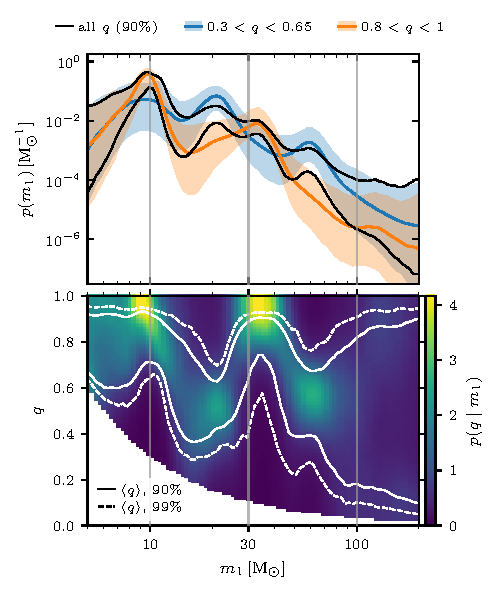
\includegraphics[width=\linewidth]{draft/plots/mass_ratio_m1.pdf}
    \caption{Top: the primary mass distribution $p(m_1)$ over all mass ratios (black lines: 90\% interval) and restricted to $0.3 < q < 0.65$ (blue) and $0.8 < q < 1$ (orange) (90\% bands and medians), for the \flexiblespins model. Bottom: the median $p(q \mid m_1)$, with the 90\% (solid) and 99\% (dashed) intervals of the mean mass ratio $\langle q \rangle$ at each $m_1$; cells with $m_2 < 3\,\Msun$ are blank.}
    \label{fig: mass}
\end{figure}

To put numbers on the peaks, we fit a simple parametric model to each posterior draw of $p(m_1, q)$ in a window $m_1 \in [m_{\rm min}, m_{\rm max}]$ around each peak:
\begin{multline}
    p(m_1, q \mid \Lambda) = \eta\, \mathrm{PL}(m_1 \mid \alpha)\, \mathcal{N}_{[0, 1]}(q \mid \mu_q', \sigma_q') \\
    + (1 - \eta)\, \mathcal{N}(m_1 \mid \mu, \sigma)\, \mathcal{N}_{[0, 1]}(q \mid \mu_q, \sigma_q),
\end{multline}
a Gaussian peak on a power-law background, each with its own truncated-Gaussian mass ratio distribution. We fit by minimizing the Kullback--Leibler divergence from the inferred $p(m_1, q)$. No mass ratio range is imposed, so each peak's mass ratio is measured, not assumed. Table~\ref{tab: peaks} and Fig.~\ref{fig: bookkeeping}(a) give the results. The locations agree between the two spin models, and with fits to the one-dimensional $p(m_1 \mid q)$ in each mass ratio range (Supplemental Material).

\begin{table}
    \caption{The four peaks: location $\mu$, width $\sigma$ and mean mass ratio $\langle q \rangle$ from the joint $(m_1, q)$ fits, for the \flexiblespins model (medians and 90\% intervals; \gaussianspins values in the Supplemental Material).}
    \label{tab: peaks}
    \begin{ruledtabular}
    \begin{tabular}{lccc}
        Peak & $\mu$ [\Msun] & $\sigma$ [\Msun] & $\langle q \rangle$ \\
        \hline
        \featTen & $\jointTenMuFlex$ & $\jointTenSigmaFlex$ & $\jointTenQMeanFlex$ \\
        \featTwenty & $\jointTwentyMuFlex$ & $\jointTwentySigmaFlex$ & $\jointTwentyQMeanFlex$ \\
        \featThirtyFive & $\jointThirtyFiveMuFlex$ & $\jointThirtyFiveSigmaFlex$ & $\jointThirtyFiveQMeanFlex$ \\
        \featSixty & $\jointSixtyMuFlex$ & $\jointSixtySigmaFlex$ & $\jointSixtyQMeanFlex$ \\
    \end{tabular}
    \end{ruledtabular}
\end{table}

Are the peaks real? A flexible model can mistake noise for structure, so we first test the feature the data constrain most directly: the swing in mass ratio. The mean mass ratio in a window around each peak is $\approx 0.83$--$0.88$ at \featTen and \featThirtyFive\,\Msun and $\approx 0.54$--$0.56$ at \featTwenty and \featSixty\,\Msun. Each of the three contrasts between neighboring peaks, $\Delta \approx 0.26$--$0.33$, is positive with probability $\qContrastTenTwentyPFlex\%$, $\qContrastThirtyFiveTwentyPFlex\%$ and $\qContrastThirtyFiveSixtyPFlex\%$ (\flexiblespins; $\qContrastTenTwentyPGauss\%$, $\qContrastThirtyFiveTwentyPGauss\%$ and $\qContrastThirtyFiveSixtyPGauss\%$ for \gaussianspins), and lies $z = \qContrastThirtyFiveSixtyZFlex$--$\qContrastThirtyFiveTwentyZFlex$ standard deviations from zero. The $m_2 > 3\,\Msun$ cut offsets $\Delta_{\featTen,\featTwenty}$ by $\approx 0.07$ under the prior; measured from the prior's center, the contrasts lie $\qContrastThirtyFiveSixtyZShiftFlex$--$\qContrastThirtyFiveTwentyZShiftFlex$ standard deviations away (Supplemental Material). Because the contrasts compare the peaks with one another, they depend neither on where a window ends nor on a model of the background. Peaks in $m_1$ itself are harder to establish. Our fits return the best Gaussian in a window whether or not a peak is there: nearly every posterior draw has one (fractions $\jointTenPeakFracFlex\%$, $\jointTwentyPeakFracFlex\%$, $\jointThirtyFivePeakFracFlex\%$ and $\jointSixtyPeakFracFlex\%$ for the \featTen, \featTwenty, \featThirtyFive and \featSixty\,\Msun peaks), but so do 70--85\% of draws from the prior. A sharper test asks whether each peak rises above a local power law, the straight line in $(\ln m_1, \ln p)$ joining the window's edges, with $p$ integrated over the peak's own mass ratio range. The excess at the most prominent bin is positive with probability $\peakTenExcessPLocFlex\%$, $\peakTwentyExcessPLocFlex\%$, $\peakThirtyFiveExcessPLocFlex\%$ and $\peakSixtyExcessPLocFlex\%$, against $\approx 0.3$--$0.6$ for the same windows in the other mass ratio range. All of these are posterior probabilities, not $p$-values, and we chose the windows after looking at the population. We therefore regard the change in mass ratio across the mass spectrum as well supported, and the $q \sim 0.5$ populations as distinct peaks in $m_1$, rather than shoulders, as tentative. A calibrated significance requires mock catalogs analyzed with the same pipeline, which we outline in the Supplemental Material.

\subsection{Peak locations: consistent with dynamical \acp{BBH}?}

If the $q \sim 0.5$ peaks are hierarchical mergers, the bookkeeping is simple. Each secondary should be a first-generation \ac{BH} from the matching equal-mass peak, and each primary the remnant of a merger of two of them. We can check both.

The secondaries line up. The typical secondary mass of each $q \sim 0.5$ peak, $\langle q \rangle \mu$, is $\approx 10$ and $\approx 32\,\Msun$ for the \featTwenty and \featSixty\,\Msun peaks, right at the equal-mass peaks. The secondary mass distribution shows plateaus rather than peaks at these masses (Fig.~\ref{fig: m2}), as it should: the width of the mass ratio distribution spreads even a narrow peak in $m_1$ over a factor of $\sim 2$ in $m_2 = q m_1$. \todo{forward-model $p(m_2)$ from the fitted peaks and compare the plateau edges}

The primaries nearly line up. A near-equal-mass merger of slowly spinning \acp{BH} radiates $\approx 5\%$ of the binary's total mass in gravitational waves~\cite{Gerosa:2021mno}, so the second-generation peak should sit at $\approx 0.95\,\mu_{\rm lo}(1 + \langle q \rangle_{\rm lo})$. We define the retained fraction
\begin{equation}
    f_{\rm ret} = \frac{\mu_{\rm hi}}{\mu_{\rm lo}(1 + \langle q \rangle_{\rm lo})},
\end{equation}
which should be $\approx 0.95$ (Fig.~\ref{fig: bookkeeping}b). For the $\featThirtyFive \to \featSixty$ pair, $f_{\rm ret} = \pairThirtyFiveSixtyRetainedFlex$, as expected. For the $\featTen \to \featTwenty$ pair, $f_{\rm ret} = \pairTenTwentyRetainedFlex$, with only $\pairTenTwentyQuantileRetainedFlex\%$ of the posterior below 0.95: the \featTwenty\,\Msun peak sits slightly heavier than hierarchical mergers of the \featTen\,\Msun population would place it. A fit-free version, using the modes of the total mass and primary mass distributions, gives $\pairTenTwentyRetainedModeFlex$ and $\pairThirtyFiveSixtyRetainedModeFlex$, and the same conclusion.

The $\featTen \to \featTwenty$ offset has several plausible explanations within the hierarchical picture. The $\sim \featTen\,\Msun$ peak is likely dominated by isolated binaries, with small and preferentially positive $\chieff$; the first-generation \acp{BH} retained in clusters need not share its mass spectrum, and may be heavier. Mass-dependent pairing in clusters also favors heavier first-generation \acp{BH}. And 0.95 is only approximate, since the radiated fraction depends on the first-generation spins and mass ratios. \todo{replace 0.95 by the distribution of remnant masses from numerical-relativity fits, averaged over the \featTen\,\Msun peak's $q$ and spin posteriors} Telling these apart requires a model with explicit formation channels, beyond the scope of this work.

\begin{figure}
    \centering
    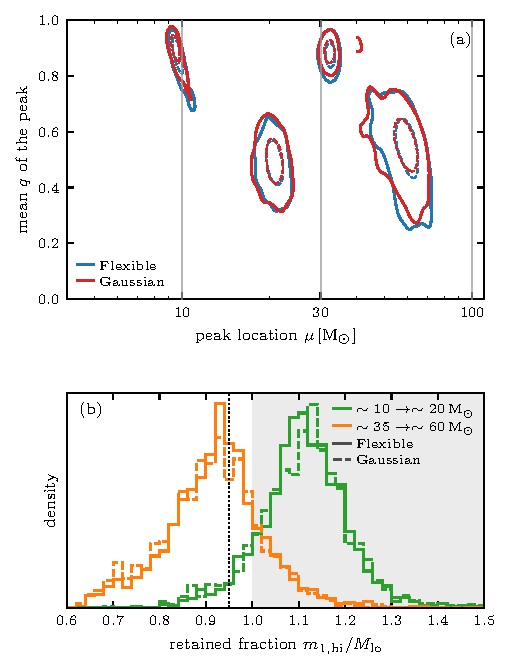
\includegraphics[width=\linewidth]{draft/plots/peak_bookkeeping.pdf}
    \caption{(a) Each peak's location $\mu$ against its mean mass ratio, from the joint $(m_1, q)$ fits; 90\% (solid) and 50\% (dashed) regions for the \flexiblespins (blue) and \gaussianspins (red) models. (b) The retained fraction $f_{\rm ret}$ for the $\featTen \to \featTwenty$ and $\featThirtyFive \to \featSixty$ pairs, from the modes of $p(m_1 \mid 0.3 < q < 0.65)$ and of the total mass of the lower peak. Dotted: 0.95 ($\sim 5\%$ radiated); shaded: $f_{\rm ret} > 1$.}
    \label{fig: bookkeeping}
\end{figure}

\section{Spin behavior}

The spins tell the same story. The width of the effective spin distribution (Fig.~\ref{fig: width m1}) is small at the equal-mass peaks, $\sim \featTen$ and $\sim \featThirtyFive\,\Msun$, and large at $\sim 18$--$20$ and $\gtrsim 45\,\Msun$, where the $q \sim 0.5$ peaks sit. The broadening comes from the unequal-mass binaries: it is absent in the $0.8 < q < 1$ slice. Both spin models agree.

\begin{figure}
    \centering
    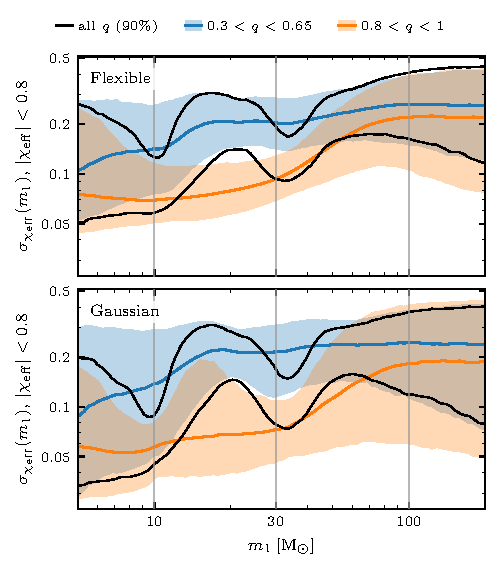
\includegraphics[width=\linewidth]{draft/plots/chi_eff_sd_m1_core.pdf}
    \caption{The width of the effective spin distribution at each primary mass, $\sigma_{\chieff}(m_1)$, the standard deviation of $p(\chieff \mid m_1, |\chieff| < 0.8)$, over all mass ratios (black lines: 90\% interval) and for $0.3 < q < 0.65$ (blue) and $0.8 < q < 1$ (orange) (90\% bands and medians), for the \flexiblespins (top) and \gaussianspins (bottom) models.}
    \label{fig: width m1}
\end{figure}

Averaged over primary mass, the broadening becomes a clean trend in mass ratio (Fig.~\ref{fig: width q}). In the \flexiblespins model, $\sigma_{\chieff} = \chiQBroadSdQLoCoreFlex$ at $q = 0.35$ and $\chiQBroadSdQHiCoreFlex$ at $q = 0.85$, a ratio of $\chiQBroadSdRatioCoreFlex$; the width is larger at $q = 0.35$ with probability $\chiQBroadProbCoreFlex\%$, against $\chiQBroadProbPriorCoreFlex\%$ under the prior. The \gaussianspins model gives $\chiQBroadSdQLoCoreGauss$ and $\chiQBroadSdQHiCoreGauss$, with probability $\chiQBroadProbCoreGauss\%$ (prior: $\chiQBroadProbPriorCoreGauss\%$). The mean of $\chieff$ barely moves with $q$ (Supplemental Material): the effective spins at low mass ratio are broader, not shifted. This agrees with the linear and spline $\chieff \mid q$ models of \citet{LIGOScientific:2026ctl}, which assume a functional form in $q$; we recover the trend without one, and localize it to the $q \sim 0.5$ peaks.

\begin{figure}
    \centering
    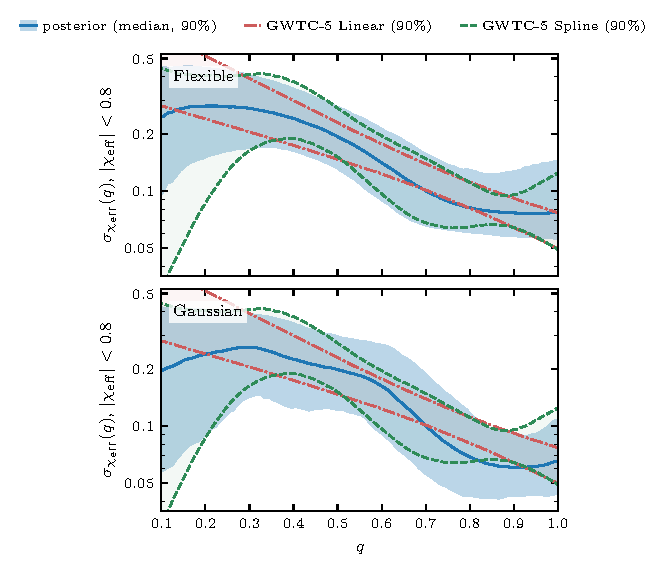
\includegraphics[width=\linewidth]{draft/plots/chi_eff_sd_q_core_lvk.pdf}
    \caption{The width of the effective spin distribution as a function of mass ratio, $\sigma_{\chieff}(q)$, averaged over $p(m_1 \mid q)$ and restricted to $|\chieff| < 0.8$, for the \flexiblespins (top) and \gaussianspins (bottom) models (blue: median and 90\% band). Lines: the 90\% intervals of $\sigma_{\chieff}(q)$ in the GWTC-5 linear (red, dash-dotted) and spline (green, dashed) $\chieff \mid q$ models~\cite{LIGOScientific:2026ctl}.}
    \label{fig: width q}
\end{figure}

Figure~\ref{fig: spin regions} shows the full $(\chieff, \chip)$ distribution in each peak region. The equal-mass peaks have narrow, slightly positive $\chieff$, as expected for first-generation \acp{BH} with small spins. The $q \sim 0.5$ peaks have broad $\chieff$, nearly symmetric about zero. This is the signature of hierarchical mergers in clusters: a near-equal-mass merger leaves a remnant spinning at $\chi \approx 0.69$, and dynamical assembly orients that spin isotropically~\cite{Gerosa:2017kvu, Fishbach:2017dwv, Rodriguez:2019huv}. Paired with a slowly spinning companion at $q \approx 0.5$, such a remnant gives $\chieff$ centered on zero with a standard deviation of $\approx 0.27$ (Supplemental Material). The measured width at $q = 0.35$, $\chiQBroadSdQLoCoreFlex$, is comparable. First-generation binaries that share the window with the $q \sim 0.5$ peaks narrow the expected width, so a quantitative comparison needs a mixture prediction. \todo{mixture prediction from the fitted peak fractions} The symmetry matters too: hierarchical mergers in active galactic nuclei disks would produce preferentially positive $\chieff$~\cite{Li:2025iux}, so a symmetric broadening favors clusters.

\begin{figure*}
    \centering
    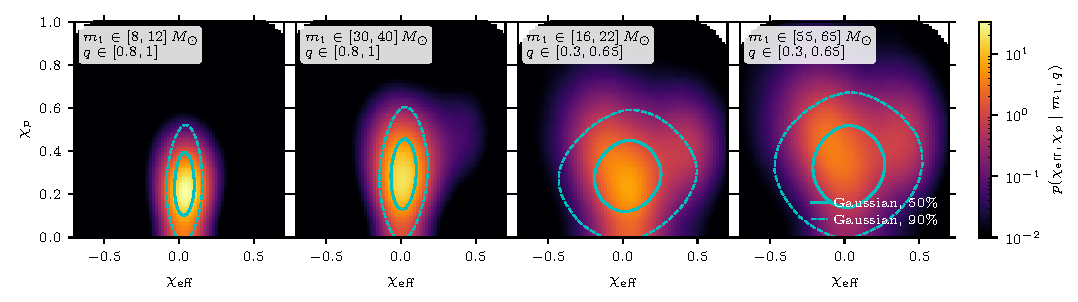
\includegraphics[width=\linewidth]{draft/plots/spin_peak_regions.pdf}
    \caption{The joint spin distribution $p(\chieff, \chip \mid m_1, q)$ in the four peak regions: the near-equal-mass peaks ($m_1 \in [8, 12]$ and $[30, 40]\,\Msun$, $q \in [0.8, 1]$) and the $q \sim 0.5$ peaks ($m_1 \in [16, 22]$ and $[55, 65]\,\Msun$, $q \in [0.3, 0.65]$). Heatmap: the \flexiblespins model's median density; contours: the \gaussianspins model's 50\% (solid) and 90\% (dashed) regions. The blank corner is outside the physical domain.}
    \label{fig: spin regions}
\end{figure*}

The precessing spin adds little. Individual $\chip$ measurements are close to their priors, especially at low mass. Averaged over mass ratio, the mean $\chip$ rises with primary mass in the \flexiblespins model, from $\approx 0.21$ at $\featTen\,\Msun$ to $\approx 0.30$ at \featTwenty and $\featThirtyFive\,\Msun$ and $\approx 0.41$ at $\featSixty\,\Msun$, and less steeply in the \gaussianspins model ($\approx 0.27$ to $0.34$), with 90\% intervals of $\pm 0.05$--$0.15$. It shows no distinct change at the $q \sim 0.5$ peaks, where hierarchical mergers alone would give $\langle \chip \rangle \approx 0.55$ (Supplemental Material). Since a poorly measured $\chip$ lets each model revert to its default, this trend is not clearly informed by the data; near the \featTwenty\,\Msun peak, the smoothness of the field likely also pulls the $\chip$ moments toward those of the more populous equal-mass peak next door. We therefore rest our conclusions on $\chieff$, and treat $\chip$ as consistent with, but not evidence for, hierarchical mergers. \todo{state the $\chip$ moments at the four peaks, with the prior for comparison}

\section{Discussion}

The \ac{BBH} population is not separable in mass and mass ratio. Once the mass ratio and spin distributions are allowed to vary across the mass spectrum, two families appear: near-equal-mass binaries peaking at $\sim \featTen$ and $\sim \featThirtyFive\,\Msun$ with narrow effective spins, and $q \sim 0.5$ binaries concentrated at about twice those masses, possibly as distinct peaks, with broad, symmetric effective spins. The $\featThirtyFive \to \featSixty$ pair matches hierarchical mergers in both mass and spin. The $\featTen \to \featTwenty$ pair matches in spin and in secondary mass, but its primary sits slightly heavier than the simplest remnant-mass estimate predicts.

Two caveats limit how far these results go. First, significance. The swing in mass ratio between the peaks is clear in the posterior, $z = \qContrastThirtyFiveSixtyZShiftFlex$--$\qContrastThirtyFiveTwentyZShiftFlex$ from the prior's center; whether the $q \sim 0.5$ binaries form distinct peaks in $m_1$ is less certain. Neither is a calibrated significance: we chose the windows after inspecting the population, and posterior probabilities from models this flexible must be calibrated with mock catalogs analyzed with the same pipeline, which we leave to future work. The full sample from the fourth observing run, roughly two to four times larger, should settle the question. Second, redshift. Our main models assume that the spin distribution is independent of redshift. When we let it vary with redshift as well as with $(m_1, q)$, we find no significant redshift dependence at fixed $(m_1, q)$ where the data constrain it, and the broadening of $\chieff$ toward low $q$ holds at all redshifts (Supplemental Material). Whether the mass distribution, and in particular the $q \sim 0.5$ peaks, evolves with redshift, as hierarchical mergers in clusters might, remains to be tested. Interpreting these features quantitatively needs a model with explicit formation channels, the subject of a companion paper.

\begin{acknowledgments}
\todo{acknowledgments, LVK data statement, computing resources}
\end{acknowledgments}

\bibliography{draft/main}

\clearpage
\onecolumngrid
\setcounter{equation}{0}
\setcounter{figure}{0}
\setcounter{table}{0}
\setcounter{section}{0}
\renewcommand{\theequation}{S\arabic{equation}}
\renewcommand{\thefigure}{S\arabic{figure}}
\renewcommand{\thetable}{S\arabic{table}}
\renewcommand{\thesection}{S\arabic{section}}

\begin{center}
\textbf{\large Supplemental Material}
\end{center}

This Supplemental Material describes the data (Sec.~\ref{sm: data}), the likelihood (Sec.~\ref{sm: likelihood}), the population models and their priors (Secs.~\ref{sm: fields}--\ref{sm: spin models}), how we evaluate them efficiently (Sec.~\ref{sm: implementation}), the sampler (Sec.~\ref{sm: sampling}), the post-processing of the posterior into spin moments (Sec.~\ref{sm: moments}), the peak fits and their significance (Secs.~\ref{sm: peak fits}--\ref{sm: significance}), the robustness tests (Sec.~\ref{sm: robustness}), and the hierarchical-merger expectations used in the main text (Sec.~\ref{sm: hierarchical}).

\section{Data}
\label{sm: data}

\textit{Events.} We use the 259 \acp{BBH} with \ac{FAR} $< 1\peryear$ in the population analysis of \citet{LIGOScientific:2026ctl}, spanning the first through fourth observing runs (O1--O4b), with the same event list, exclusions and waveform choices. The \ac{PE} samples come from the GWTC-2.1 and GWTC-3 data releases for O1--O3 and from the GWTC-4 and GWTC-5 releases for O4a and O4b. For each event we take the first available of NRSur7dq4~\cite{Varma:2019csw}, the mixed-waveform samples, and IMRPhenomXPHM-SpinTaylor~\cite{Pratten:2020ceb}. The list excludes sub-threshold events and events with a possible neutron star, including GW190814 and GW190917. Each sample carries its \ac{PE} prior density, which we convert to $(\ln m_1, q, \chieff, \chip, z)$, including the Jacobians of the transformation. \todo{cite the data releases}

\textit{Sensitivity.} We estimate the selection function with the mixture of sensitivity injections released with \ac{GWTC-5}: real-noise injections for O3, O4a and O4b and semianalytic injections for O1 and O2, with the same detection threshold as the events (\ac{FAR} $< 1\peryear$, and a network signal-to-noise ratio above 10 for the semianalytic injections).

\textit{Domain.} Samples and injections are restricted to $m_1 \in [3, 200]\,\Msun$ and $z < 1.9$. Samples outside this domain are given zero weight (an infinite \ac{PE} prior), and injections outside it are removed.

\textit{Sample selection.} The number of \ac{PE} samples differs between events. We keep at most 20000 samples per event, drawn at random from the \emph{usable} samples: those inside the population grid, in a $(\ln m_1, q)$ bin and a $(\chieff, \chip)$ bin that at least one detected injection reaches. Samples that are not usable carry zero weight in the likelihood anyway, since the population density at an unreachable bin cannot be constrained by the selection function. Leaving them out of the count shifts each event's log-likelihood by the constant $-\ln(N_{\rm usable}/N_{\rm real})$, which does not affect inference. Over the catalog, a fraction $9.7 \times 10^{-4}$ of samples is not usable, at most 2.3\% for one event (GW230704, mostly at $z > 1.9$). Events with fewer samples are padded to a rectangular array with zero-weight copies, and the per-event sample count is kept for the Monte Carlo estimators below.

\section{Likelihood}
\label{sm: likelihood}

For hyperparameters $\Lambda$, we write the population as a density $p(\theta \mid \Lambda)$ over $\theta = (\ln m_1, q, \chieff, \chip, z)$ and the merger rate as $R\, p(\theta \mid \Lambda)$. Marginalizing over $R$ with a scale-invariant prior gives the standard hierarchical likelihood~\cite{Mandel:2018mve, Thrane:2018qnx}
\begin{equation}
    \ln \mathcal{L}(\Lambda) = \sum_{i=1}^{N_{\rm obs}} \ln \hat{\mathcal{L}}_i(\Lambda) - N_{\rm obs} \ln \hat{\xi}(\Lambda),
\end{equation}
with the Monte Carlo estimates
\begin{equation}
    \hat{\mathcal{L}}_i = \frac{1}{M_i} \sum_{j=1}^{M_i} w_{ij}, \quad w_{ij} = \frac{p(\theta_{ij} \mid \Lambda)}{\pi_i(\theta_{ij})}, \qquad
    \hat{\xi} = \frac{1}{T} \sum_{k\,\in\,\rm found} w_k, \quad w_k = \frac{p(\theta_k \mid \Lambda)}{p_{\rm draw}(\theta_k)},
\end{equation}
where $\theta_{ij}$ are the $M_i$ samples of event $i$ with \ac{PE} prior $\pi_i$, and $\theta_k$ the found injections out of $T$ generated, with draw density $p_{\rm draw}$. Both weights include the redshift factor $\frac{dV_c}{dz} \frac{1}{1+z} (1 + z)^{\lambda}$.

\textit{Monte Carlo uncertainty.} The variance of the log-likelihood estimate is
\begin{equation}
    \sigma^2_{\ln \mathcal{L}} = \sum_i \frac{1}{N_{{\rm eff}, i}} + \frac{N_{\rm obs}^2}{N_{\rm eff, sel}}, \qquad
    N_{{\rm eff}, i} = \left[\frac{\sum_j w_{ij}^2}{(\sum_j w_{ij})^2} - \frac{1}{M_i}\right]^{-1},
\end{equation}
with the analogous effective sample size $N_{\rm eff, sel}$ for the injections~\cite{Farr:2019rap, Essick:2022ojx, Talbot:2023pex}. We record it, with its per-event and selection parts, at every posterior sample. We impose no cut on $\sigma^2_{\ln\mathcal{L}}$.

\textit{Per-event effective sample size.} Flexible models can place structure on scales smaller than an event's \ac{PE} samples resolve, where $\hat{\mathcal{L}}_i$ becomes unreliable. We therefore require $N_{{\rm eff}, i} \geq 100$ for every event, imposed as a smooth penalty, $\sum_i s(-\ln N_{{\rm eff}, i};\, -\ln 100,\, 0.1)$, where $s(x; x_0, \delta)$ is a smoothed step from zero to a large negative value at $x_0$ with width $\delta$. A smooth penalty keeps the log density differentiable for the sampler.

\textit{Selection bias correction.} $1/\hat{\xi}^{N_{\rm obs}}$ is a biased estimate of $1/\xi^{N_{\rm obs}}$. To leading order, its expectation is too large by a factor $1 + N_{\rm obs}(N_{\rm obs} + 1)\sigma_{\rm sel}^2/2$, with
\begin{equation}
    \sigma_{\rm sel}^2 = \frac{1}{T - 1}\left[T\frac{\sum_k w_k^2}{(\sum_k w_k)^2} - 1\right].
\end{equation}
Following \citet{Heinzel:2025ogf}, we subtract $N_{\rm obs}(N_{\rm obs} + 1)\sigma^2_{\rm sel}/2$ from $\ln \mathcal{L}$.

\textit{Monte Carlo systematics.} To check that the Monte Carlo error does not drive our results, we estimate for each reported quantity $f$ the systematic shift of its posterior mean due to the Monte Carlo error of $\ln \hat{\mathcal{L}}$. To first order, the spread of this shift over Monte Carlo realizations is
\begin{equation}
    \sigma^2_{\rm syst} = \frac{1}{N^2} \sum_{n, m} \delta f_n\, \delta f_m\, C(\Lambda_n, \Lambda_m), \qquad \delta f_n = f(\Lambda_n) - \overline{f},
\end{equation}
where $C$ is the covariance of the log-likelihood error between posterior samples $\Lambda_n$ and $\Lambda_m$~\cite{Heinzel:2025ogf}. Writing $C$ as a sum over \ac{PE} samples and injections of products of normalized weights reduces this to a single pass over the posterior samples, $\sigma^2_{\rm syst} = \sum_s c_s g_s^2$ with $g_s = N^{-1}\sum_n \delta f_n \tilde{w}_{n, s}$, where $c_s = 1/[M_i(M_i - 1)]$ for the samples of event $i$ and $N_{\rm obs}^2/[T(T - 1)]$ for the injections. We compare $\sigma_{\rm syst}$ with the posterior standard deviation $\sigma_{\rm stat}$. \todo{$\sigma_{\rm syst}/\sigma_{\rm stat}$ for the peak locations, $f_{\rm ret}$ and $\sigma_{\chieff}(q)$}

\section{Mat\'ern fields}
\label{sm: fields}

All population fields are Mat\'ern Gaussian random fields on a regular grid, represented in the Laplacian eigenbasis of the grid, following the stochastic partial differential equation construction~\cite{Whittle:1954abc, lindgren_explicit_2011} used in \PixelPop~\cite{Heinzel:2024jlc}.

\textit{Eigenbasis.} Along each axis $d$ with $B_d$ bins, we take the graph Laplacian of the path graph (each bin coupled to its neighbors), and its eigenvectors $v^{(d)}_k$ and eigenvalues $\lambda^{(d)}_k$, $k = 0, \dots, B_d - 1$, with $\lambda^{(d)}_0 = 0$ for the constant mode. On a $D$-dimensional grid, the products $\prod_d v^{(d)}_{k_d}$ form an orthonormal basis.

\textit{Field.} A field is
\begin{equation}
    f = \sum_{\vec{k}} a_{\vec{k}}\, z_{\vec{k}} \prod_{d=1}^{D} v^{(d)}_{k_d}, \qquad z_{\vec{k}} \sim \mathcal{N}(0, 1),
\end{equation}
with the Mat\'ern spectrum
\begin{equation}
    a_{\vec{k}} = s \sqrt{\frac{N_{\rm sites}}{\sum_{\vec{k}'} \tilde{a}_{\vec{k}'}^2}}\; \tilde{a}_{\vec{k}}, \qquad
    \tilde{a}_{\vec{k}} = \Big(1 + \sum_{d} \frac{\ell_d^2\, \lambda^{(d)}_{k_d}}{8\nu}\Big)^{-(\nu + D/2)/2},
\end{equation}
where $\ell_d$ is the range along axis $d$ in bins, $\nu$ the smoothness and $N_{\rm sites}$ the number of grid sites. The normalization makes the site-averaged variance of $f$ equal to $s^2$, independent of $\ell_d$ and $\nu$, so the amplitude and the correlation structure are separately identified. The constant mode $\vec{k} = 0$ is set to zero: it is degenerate with the normalization of the density.

\textit{Parametrization.} We sample the white-noise coefficients $z_{\vec{k}}$ and the hyperparameters $(s, \nu, \ell_d)$, not the field itself (a non-centered parametrization), which removes the strong posterior correlation between the field and its amplitude~\cite{Papaspiliopoulos:2007abc, Betancourt:2017ebh}.

\textit{Hyperpriors.} Unless stated otherwise, $\ln s \sim \mathcal{N}(0, 2)$, $\ln \nu \sim \mathcal{N}(0, 0.5)$, and $\ln \ell_d \sim \mathcal{U}(0, \ln B_d)$, log-uniform from one bin to the length of the axis; these are the \PixelPop defaults.

\section{Mass and redshift model}
\label{sm: mass model}

The mass distribution is
\begin{equation}
    p(\ln m_1, q) \propto e^{L(\ln m_1, q)}\, \Theta(q m_1 - 3\,\Msun),
\end{equation}
with $L$ a two-dimensional Mat\'ern field on $100 \times 100$ bins uniform in $\ln m_1 \in [\ln 3, \ln 200]$ and $q \in [0, 1]$, keeping all $10^4$ modes, and piecewise constant within each bin. The step function, the $m_2 > 3\,\Msun$ window, is applied as a separate factor, with its lower edge fixed at $3\,\Msun$ and no tapering. All mass distributions we show are windowed and renormalized; the field $L$ alone is not.

The redshift distribution is $p(z) \propto \frac{dV_c}{dz} \frac{1}{1+z} (1 + z)^{\lambda}$ on $z < 1.9$, independent of mass and spin, with $\lambda \sim \mathcal{U}(-10, 10)$.

\section{Spin models}
\label{sm: spin models}

\textit{Physical domain.} For given $q$ and $\chieff$, the largest reachable $\chip$, with component spin magnitudes below 1, is~\cite{iwaya_analytic_2025}
\begin{equation}
    \chi_{\rm p, max}(\chieff, q) = \sqrt{1 - x^2}, \qquad x = \min\big[\max\big((1 + q)|\chieff| - q,\, 0\big),\, 1\big].
\end{equation}
The spin distribution lives on $100 \times 100$ bins uniform over $\chieff \in [-1, 1]$ and $\chip \in [0, 1]$, restricted to $\chip < \chi_{\rm p, max}(\chieff, q)$. Many bins are cut by this boundary. For each $(\chieff, \chip)$ bin and each $q$ bin, we compute the allowed fraction $f_b(q)$ of the bin's area, on 64 sub-bins in $\chieff$ and 8 values of $q$ across the $q$ bin. A spin density that is constant within a bin then has total probability $\propto e^{F_b} f_b$ in it. The fraction enters the normalization only, so a sample's density is the same anywhere in its bin.

\textit{Normalization.} Each spin model gives a log density $F(\ln m_1, q, \chieff, \chip)$ on the grid, and
\begin{equation}
    \ln p(\chieff, \chip \mid m_1, q) = F - \ln Z(m_1, q), \qquad \ln Z = \LSE_{b}\big[F_b + \ln f_b(q)\big],
\end{equation}
with $\LSE$ the log-sum-exp over spin bins. Bins that no $q$ in the $q$ bin can reach ($f_b = 0$) are assigned a log density of $-10^4$ instead of $-\infty$, which gives them zero probability while keeping all gradients finite. \ac{PE} samples or injections in bins with $f_b = 0$ would have zero weight. \todo{confirm that there are none} We also give zero weight to the (few) \ac{PE} samples in spin bins that no detected injection reaches.

\textit{The} \flexiblespins \textit{model.} $F$ is a four-dimensional Mat\'ern field, factorized over the mass plane:
\begin{equation}
    F(\ln m_1, q, \chi) = \sum_{k, l < K} v^{(m)}_k(\ln m_1)\, v^{(q)}_l(q)\, G_{kl}(\chieff, \chip),
\end{equation}
keeping the $K = 10$ lowest modes along each mass axis and all $100 \times 100$ spin modes. $G$ has the Mat\'ern spectrum of Sec.~\ref{sm: fields} in four dimensions, with a single amplitude $s$, a single smoothness $\nu$ and four ranges. The mass ranges have the default prior. The spin ranges are bounded below by $0.05$ in $\chi$, that is 2.5 bins in $\chieff$ and 5 bins in $\chip$, so that the spin distribution cannot vary on scales finer than individual events resolve. Modes that are constant in $\chi$ (the $(0, 0)$ spin mode of every mass mode) add a function of $(m_1, q)$ alone to $F$, which cancels in the normalization; we set them to zero. A field of zero is uniform on the physical domain, so the model has no preferred spin distribution. The truncation to $K = 10$ mass modes limits the spin distribution to vary on scales of about a tenth of each mass axis, about $0.4$ in $\ln m_1$ and $0.1$ in $q$, and makes the model tractable (Sec.~\ref{sm: implementation}).

\textit{The} \gaussianspins \textit{model.} The spin distribution is a bivariate Gaussian in $(\chieff, \chip)$, truncated to the physical domain and normalized at each $(m_1, q)$ as above:
\begin{equation}
    F = -\frac{1}{2(1 - \rho^2)}\left[x^2 - 2\rho x y + y^2\right] - \ln(\sigma_{\chieff} \sigma_{\chip}) - \frac{1}{2}\ln(1 - \rho^2), \qquad
    x = \frac{\chieff - \mu_{\chieff}}{\sigma_{\chieff}}, \quad y = \frac{\chip - \mu_{\chip}}{\sigma_{\chip}},
\end{equation}
that is, $p \propto \mathcal{N}(\vec{\mu}, C)$ with
\begin{align}
    \vec{\mu} &= \begin{bmatrix} \mu_{\chieff} \\ \mu_{\chip} \end{bmatrix}, &
    C &= \begin{bmatrix}
    \sigma^2_{\chieff} & \rho\,\sigma_{\chieff}\sigma_{\chip} \\
    \rho\,\sigma_{\chieff}\sigma_{\chip} & \sigma^2_{\chip}
    \end{bmatrix}, \label{eq: gaussian cov}
\end{align}
each entry a function of $(m_1, q)$. The five parameters $\theta_i \in \{\mu_{\chieff}, \mu_{\chip}, \ln\tilde{\sigma}_{\chieff}, \ln\tilde{\sigma}_{\chip}, \operatorname{atanh}\rho\}$ are each a constant plus a two-dimensional Mat\'ern field over the $(\ln m_1, q)$ grid, $\theta_i = c_i + f_i(\ln m_1, q)$, with the constant mode of $f_i$ set to zero so that $c_i$ carries the mean. Each $f_i$ has its own amplitude $s_i$ and ranges, and the smoothness $\nu$ is shared. We use all $100 \times 100$ mass modes ($5 \times 10^4$ white-noise coefficients). The widths entering the Gaussian are $\sigma = (\tilde{\sigma}^2 + 0.02^2)^{1/2}$, a soft floor at one spin bin, so that the Gaussian cannot become narrower than the grid resolves. The priors are
\begin{gather}
    c_{\mu_{\chieff}} \sim \mathcal{U}(-0.5, 0.5), \quad c_{\mu_{\chip}} \sim \mathcal{U}(0, 1), \quad c_{\ln\tilde{\sigma}} \sim \mathcal{U}(\ln 0.03, 0) \text{ (both widths)}, \quad c_{\operatorname{atanh}\rho} \sim \mathcal{U}(-2, 2), \\
    \ln s_i \sim \mathcal{N}(\ln 0.1, 1) \text{ for the two means}, \qquad \ln s_i \sim \mathcal{N}(\ln 0.5, 1) \text{ for the two log-widths and } \operatorname{atanh}\rho,
\end{gather}
and the default priors on $\nu$ and the ranges. The amplitude priors are centered on the scale over which each parameter can plausibly vary across the mass plane: $\sim 0.1$ in the means, and a factor of $\sim e^{0.5}$ in the widths.

\textit{The split model (robustness).} $F = G_0(\chi) + G_1(\ln m_1, q, \chi)$. $G_0$ is a mass-independent two-dimensional Mat\'ern field on $(\chieff, \chip)$ with its own $(s_0, \nu_0, \ell)$. $G_1$ keeps the $10 \times 10$ mass modes except the constant one, with its own amplitude $s_1$ and smoothness $\nu_1$, and a separable spectrum: the product of a two-dimensional Mat\'ern spectrum over the mass modes and one over the spin modes, each with the constant mode removed. Variations of the spin distribution along mass are then not damped jointly with variations in $\chi$, and $s_1$ directly measures how much the spin distribution changes with mass. Since the lowest mass eigenvectors are constant, $G_0$ enters as a constant addition to the $(0, 0)$ mass mode.

\section{Implementation}
\label{sm: implementation}

The model is written in \textsc{JAX} and \textsc{NumPyro}~\cite{Phan:2019numpyro} and runs on a single GPU. The four-dimensional spin density of the \flexiblespins model has $100^4 = 10^8$ cells, too many to form at once, and the population density must be evaluated at more than $5 \times 10^6$ \ac{PE} samples and injections, with gradients, at every sampler step. We make this tractable as follows.

\textit{Factorization.} The \flexiblespins field is stored as its $10 \times 10 \times 100 \times 100$ coefficients $G_{kl}(\chi)$ in the mass eigenbasis and spin grid. At a sample in bin $(a, b, c, d)$ of $(\ln m_1, q, \chieff, \chip)$, $F = \sum_{kl} v^{(m)}_k(a)\, v^{(q)}_l(b)\, G_{kl}(c, d)$, a contraction over 100 coefficients that never forms the full cube.

\textit{Normalization by slabs.} The normalization $\ln Z(m_1, q)$ requires a log-sum-exp over all spin bins at every mass cell. We compute it one $\ln m_1$ bin at a time, forming the $100 \times 100 \times 100$ slab of $(q, \chieff, \chip)$, with a sequential map over the 100 slabs (in batches of 10). Each slab is rematerialized on the backward pass rather than stored (gradient checkpointing), so memory scales with one slab rather than with the cube. The same pass accumulates, at no extra cost, the per-cell means and standard deviations of $\chieff$ and $\chip$ and the population spin marginal, which we store at every posterior sample. The moments restricted to $|\chieff| < 0.8$ are computed afterwards from the saved fields (Sec.~\ref{sm: moments}).

\textit{Gaussian model.} The \gaussianspins density is evaluated in closed form at each sample and normalized by the same slab pass, so its cost is similar despite using all $10^4$ mass modes per parameter field.

\textit{Cost.} One evaluation of the log density and its gradient takes $\sim 25$\,ms on an NVIDIA A100 for the \flexiblespins model. \todo{update timings for the final runs}

\section{Sampling}
\label{sm: sampling}

We sample all latent variables jointly with the No-U-Turn Sampler~\cite{Hoffman:2014nuts}, with a target acceptance probability of 0.7 and a maximum tree depth of 7. The mass matrix is diagonal for the white-noise coefficients and dense within each field's hyperparameters (its amplitude, smoothness and ranges), where the posterior correlations are strongest. Each chain runs 4000 warm-up steps, during which the step size and mass matrix are adapted, followed by 5000 steps thinned by a factor of 5 to 1000 retained samples. Each chain starts from an independent random draw of the full prior, keyed by the chain index, rather than from a tuned starting point, so that agreement between chains is a meaningful convergence test. Before each run we evaluate the likelihood, its variance and the smallest per-event effective sample size at the starting point. \todo{$\hat{R}$ and effective sample sizes of the hyperparameters and of the reported quantities}

A few chains stalled early in warm-up: their step size fell from $\sim 10^{-2}$ to $\sim 10^{-6}$ with the parameters far from the posterior. The variance of the likelihood and the per-event effective sample sizes at the starting point did not predict which chains would stall. We discard these chains and replace them with new chains from different prior draws. \todo{state the agreement between the retained chains}

\section{Spin moments}
\label{sm: moments}

\textit{Per-cell moments.} At each posterior sample and each $(m_1, q)$ cell, we compute the mean and standard deviation of $\chieff$ and $\chip$ under $p(\chieff, \chip \mid m_1, q)$, on the bin centers. Because individual-event $\chieff$ measurements rarely reach $|\chieff| > 0.8$, the tails of the spin distribution there are set mostly by the prior, and can dominate a standard deviation without being constrained. We therefore also compute the \emph{core} moments, of $p(\chieff \mid m_1, q, |\chieff| < 0.8)$, together with the probability outside the core.

\textit{Moments as a function of $m_1$ or $q$.} To show the spin distribution as a function of $m_1$ alone, we average the conditional over the windowed $p(q \mid m_1)$, optionally restricted to a range of $q$. By the law of total variance,
\begin{equation}
    \sigma^2_{\chieff}(m_1) = \underbrace{\mathbb{E}_{q \mid m_1}\big[\sigma^2_{\chieff}(m_1, q)\big]}_{\rm within} + \underbrace{\mathrm{Var}_{q \mid m_1}\big[\mu_{\chieff}(m_1, q)\big]}_{\rm between},
\end{equation}
and we track both terms. The broadening at $\sim 18$--$20$ and $\gtrsim 45\,\Msun$ comes almost entirely from the \lq\lq within'' term at low $q$: the spin distribution at fixed low mass ratio is broad, rather than shifting with $q$. For core moments, each cell is additionally weighted by its probability inside the core, so the average is over $p(\chieff \mid m_1, |\chieff| < 0.8)$. The moments as a function of $q$ are computed in the same way, averaging over $p(m_1 \mid q)$.

\textit{Prior comparison.} To ask whether a spin moment is informed by the data beyond the prior, we compare it with an empirical-Bayes prior. For 2000 posterior samples, we keep the hyperparameters of the spin model and the mass field, and draw the spin white-noise coefficients afresh from $\mathcal{N}(0, 1)$ (and, for the \gaussianspins model, the constants $c_i$ from their priors). We then compute the same moments. These prior draws share the posterior's $p(q \mid m_1)$ and smoothness, so only the spin field itself is drawn from the prior.

\textit{Comparison with \ac{GWTC-5}.} For Fig.~\ref{fig: width q}, we take the posterior of the Gaussian width $\sigma_{\chieff}(q)$ of the linear and spline mass-ratio-dependent spin models of \citet{LIGOScientific:2026ctl} from their released population summaries. These widths are not restricted to $|\chieff| < 0.8$, so the comparison is approximate where the tails matter.

\section{Peak fits}
\label{sm: peak fits}

\textit{Windows.} The peaks are fitted in windows chosen by eye: $m_1 \in [5, 15]$, $[15, 30]$, $[25, 40]$ and $[40, 100]\,\Msun$ for the \featTen, \featTwenty, \featThirtyFive and \featSixty\,\Msun peaks, with the mass ratio range $0.8 < q < 1$ for the \featTen and \featThirtyFive\,\Msun peaks and $0.3 < q < 0.65$ for the \featTwenty and \featSixty\,\Msun peaks where a range is used.

\textit{Objective.} We fit each posterior sample's density $p$ by a model $f$ by minimizing the generalized Kullback--Leibler divergence over the window's cells,
\begin{equation}
    D(p \,\|\, f) = \sum_{\rm cells} a \left[p \ln\frac{p}{f} - p + f\right],
\end{equation}
with $a$ the cell area. This is the cross entropy $-\sum a\, p \ln f$ with the normalization of $f$ free, equivalent to a Poisson likelihood. Least squares in $\ln p$ gives equal weight to the many low-density cells and lets them dominate the fit; $D$ weights cells by their probability. We minimize $D$ by nonlinear least squares on the deviance residuals $\mathrm{sign}(f - p)\sqrt{2a[p\ln(p/f) - p + f]}$.

\textit{One-dimensional fits.} On $p(m_1 \mid q \in Q)$ we fit $f(m_1) = A e^{-(m_1 - \mu)^2/2\sigma^2} + B(m_1/m_{\rm ref})^{-\alpha}$, with $m_{\rm ref}$ the window's center, $\mu$ bounded to the window, $\sigma$ to $(0.03, 1)$ times its width and $\alpha$ to $(-20, 20)$. Each sample starts from two initial points, with the Gaussian at the window's maximum and at its center, and keeps the better fit.

\textit{Joint fits.} On the windowed $p(m_1, q)$ over all $q$ allowed by $m_2 > 3\,\Msun$, we fit
\begin{equation}
    f(m_1, q) = A\, \mathcal{N}(m_1; \mu, \sigma)\, \mathcal{T}(q; \mu_q, \sigma_q) + B \Big(\frac{m_1}{m_{\rm ref}}\Big)^{-\alpha} \mathcal{T}(q; \mu_q', \sigma_q'),
\end{equation}
where $\mathcal{T}$ is a Gaussian truncated to $[3\,\Msun/m_1, 1]$ and normalized at each $m_1$. The bounds are as above, with $\mu_q, \mu_q' \in (0, 1)$ and $\sigma_q \in (0.02, 3)$. The objective has local minima with the Gaussian at a window edge, so each sample starts from six initial points and keeps the lowest divergence. The reported mass ratio of a peak, $\langle q \rangle$, is the mean of $\mathcal{T}(q; \mu_q, \sigma_q)$ on $[3\,\Msun/\mu, 1]$, which unlike $\mu_q$ cannot sit on the boundary.

\textit{Samples without a peak.} A fit that fails, or ends with $\mu$ or $\sigma$ on a bound, has no peak in the window. We count these samples and exclude them from the summaries, so the reported peak parameters are conditional on a peak. Table~\ref{tab: fits} lists the results for both spin models.

\begin{table}
    \caption{Peak fits for both spin models (medians and 90\% intervals). Joint: the joint $(m_1, q)$ fits; 1D: fits to $p(m_1 \mid q \in Q)$ in each peak's mass ratio range.}
    \label{tab: fits}
    \begin{ruledtabular}
    \begin{tabular}{lcccccc}
        & \multicolumn{3}{c}{\flexiblespins} & \multicolumn{3}{c}{\gaussianspins} \\
        Peak & $\mu$ (joint) & $\langle q \rangle$ (joint) & $\mu$ (1D) & $\mu$ (joint) & $\langle q \rangle$ (joint) & $\mu$ (1D) \\
        \hline
        \featTen & $\jointTenMuFlex$ & $\jointTenQMeanFlex$ & $\peakTenMuFlex$ & $\jointTenMuGauss$ & $\jointTenQMeanGauss$ & $\peakTenMuGauss$ \\
        \featTwenty & $\jointTwentyMuFlex$ & $\jointTwentyQMeanFlex$ & $\peakTwentyMuFlex$ & $\jointTwentyMuGauss$ & $\jointTwentyQMeanGauss$ & $\peakTwentyMuGauss$ \\
        \featThirtyFive & $\jointThirtyFiveMuFlex$ & $\jointThirtyFiveQMeanFlex$ & $\peakThirtyFiveMuFlex$ & $\jointThirtyFiveMuGauss$ & $\jointThirtyFiveQMeanGauss$ & $\peakThirtyFiveMuGauss$ \\
        \featSixty & $\jointSixtyMuFlex$ & $\jointSixtyQMeanFlex$ & $\peakSixtyMuFlex$ & $\jointSixtyMuGauss$ & $\jointSixtyQMeanGauss$ & $\peakSixtyMuGauss$ \\
    \end{tabular}
    \end{ruledtabular}
\end{table}

\textit{Mass bookkeeping.} For each pair of peaks, (\featTen, \featTwenty) and (\featThirtyFive, \featSixty), we compute $f_{\rm ret} = \mu_{\rm hi}/[\mu_{\rm lo}(1 + \langle q \rangle_{\rm lo})]$ from the joint fits of the same posterior sample, so that correlations between the peaks carry through; samples without a peak in either window are dropped. We also report the location ratio $\mu_{\rm hi}/\mu_{\rm lo}$: $\pairTenTwentyLocRatioFlex$ and $\pairThirtyFiveSixtyLocRatioFlex$. The fit-free version replaces the fitted quantities by modes: the lower peak's total mass is the mode of $p(M \mid q \in Q_{\rm lo})$, $M = m_1(1 + q)$, computed by splitting each $(\ln m_1, q)$ cell into $4 \times 4$ sub-cells and binning in $\ln M$; the higher peak's location is the mode of $p(m_1 \mid q \in Q_{\rm hi})$. Each mode is the maximum of $\ln p$, refined by a parabola, within a search window ($[12, 30]$ and $[15, 30]\,\Msun$ for the \featTen--\featTwenty pair; $[45, 85]$ and $[40, 100]\,\Msun$ for the \featThirtyFive--\featSixty pair); samples whose maximum is at a window edge are dropped.

\begin{figure}
    \centering
    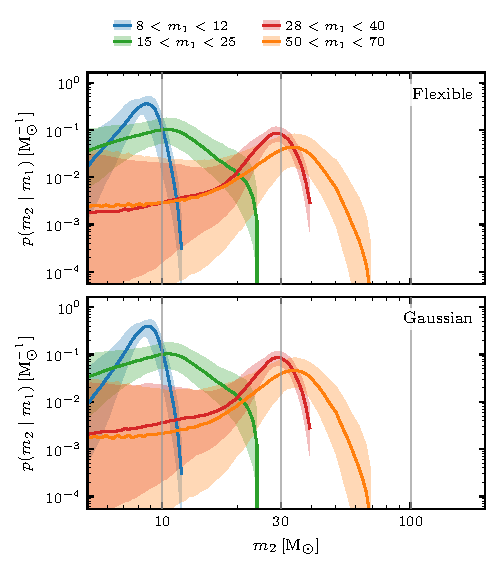
\includegraphics[width=0.6\linewidth]{draft/plots/m2_m1_windows.pdf}
    \caption{The secondary mass distribution $p(m_2 \mid m_1)$ in windows around the \featTwenty and \featSixty\,\Msun peaks, for the \flexiblespins model. The $q \sim 0.5$ peaks map onto plateaus, not peaks, in $m_2$, because the width of their mass ratio distribution spreads a narrow peak in $m_1$ over a factor of $\sim 2$ in $m_2$. \todo{describe the bands}}
    \label{fig: m2}
\end{figure}

\section{Significance of the peaks}
\label{sm: significance}

\textit{Excess over a local power law.} For each posterior sample, we take $p(\ln m_1, q \in Q)$, the windowed mass density summed over the $q$ bins of $Q$, and in each window draw the chord in $(\ln m_1, \ln p)$ between the centers of the window's first and last bins, a local power law. The excess is
\begin{equation}
    d(m_1) = \ln p(\ln m_1, q \in Q) - \mathrm{chord}(\ln m_1),
\end{equation}
which is independent of the normalization of $p$ within $Q$, and the same for densities in $m_1$ or $\ln m_1$, since these differ by a term linear in $\ln m_1$ that the chord absorbs. We report $P_{\rm loc}$, the fraction of samples with $d > 0$ at a fixed bin, the interior bin where the median of $d$ is largest. Table~\ref{tab: excess} lists these, the height and location of the maximum excess, and the signed integrated excess $F_{\rm int} = \sum_{\rm bins}(p - e^{\rm chord}) / \sum_{\rm bins} p$. The $m_2 > 3\,\Msun$ cut removes part of the low-$m_1$ end of the window at low $q$; so that the cut cannot create a rising edge, we keep only the bins where every $q$ bin of $Q$ is allowed, i.e.\ $m_1 \min Q \geq 3\,\Msun$.

\begin{table}
    \caption{Excess over a local power law, each peak in its own mass ratio range (\flexiblespins model; medians and 90\% intervals). $P_{\rm loc}$: posterior probability of a positive excess at the most prominent bin; $d_{\max}$: the maximum excess in $\ln p$; $\hat{m}$: its location; $F_{\rm int}$: the signed integrated excess fraction.}
    \label{tab: excess}
    \begin{ruledtabular}
    \begin{tabular}{lcccc}
        Peak & $P_{\rm loc}$ & $d_{\max}$ & $\hat{m}$ [\Msun] & $F_{\rm int}$ \\
        \hline
        \featTen & $\peakTenExcessPLocFlex\%$ & $\peakTenExcessHeightFlex$ & $\peakTenExcessLocFlex$ & $\peakTenExcessFIntFlex$ \\
        \featTwenty & $\peakTwentyExcessPLocFlex\%$ & $\peakTwentyExcessHeightFlex$ & $\peakTwentyExcessLocFlex$ & $\peakTwentyExcessFIntFlex$ \\
        \featThirtyFive & $\peakThirtyFiveExcessPLocFlex\%$ & $\peakThirtyFiveExcessHeightFlex$ & $\peakThirtyFiveExcessLocFlex$ & $\peakThirtyFiveExcessFIntFlex$ \\
        \featSixty & $\peakSixtyExcessPLocFlex\%$ & $\peakSixtyExcessHeightFlex$ & $\peakSixtyExcessLocFlex$ & $\peakSixtyExcessFIntFlex$ \\
    \end{tabular}
    \end{ruledtabular}
\end{table}

\begin{figure}
    \centering
    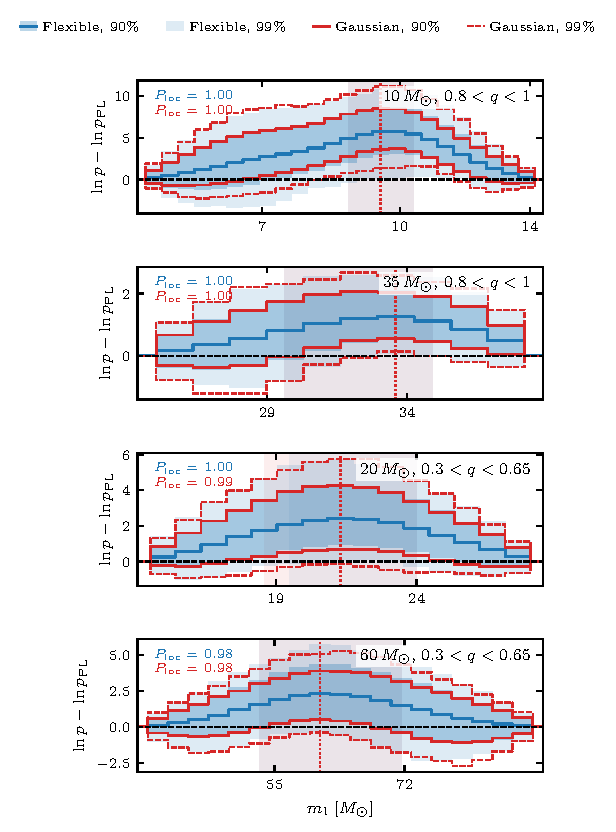
\includegraphics[width=0.6\linewidth]{draft/plots/peak_excess_own_q.pdf}
    \caption{The excess $d(m_1)$ for each peak in its own mass ratio range, per posterior sample, for the \flexiblespins (blue: 90\% and 99\% bands, median) and \gaussianspins (red: 90\% solid, 99\% dashed) models.}
    \label{fig: excess}
\end{figure}

\begin{figure}
    \centering
    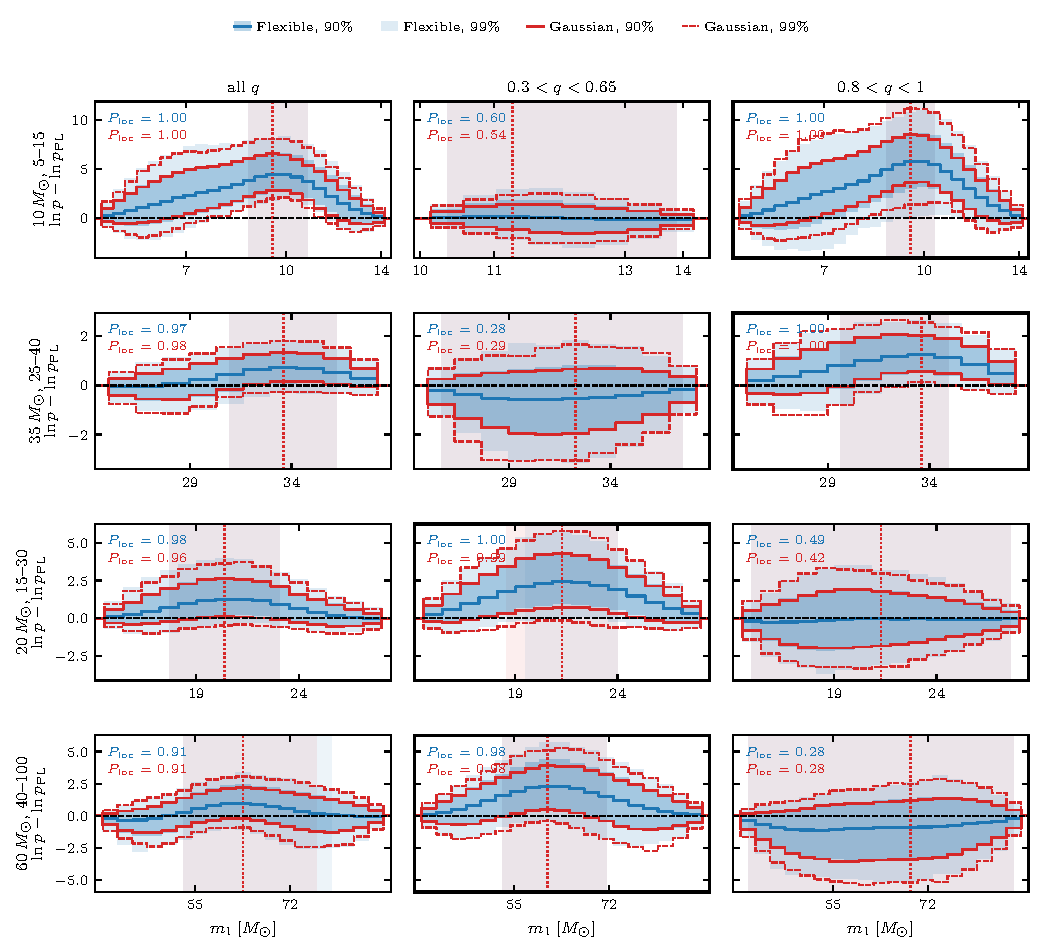
\includegraphics[width=\linewidth]{draft/plots/peak_excess.pdf}
    \caption{As Fig.~\ref{fig: excess}, for every peak window (rows) in every mass ratio range (columns: all $q$, $0.3 < q < 0.65$, $0.8 < q < 1$); boxed: each peak's own mass ratio range. The excess appears only in the boxed panels; the others show what the statistic gives without a feature.}
    \label{fig: excess grid}
\end{figure}

\textit{Mass ratio contrast.} The most direct feature in Figs.~\ref{fig: mass} and~\ref{fig: m2} is not a peak in $m_1$ but the change in the mass ratio distribution with $m_1$: near-equal masses at \featTen and \featThirtyFive\,\Msun, unequal masses at \featTwenty and \featSixty\,\Msun. In the $q \sim 0.5$ range, a peak in $p(m_1, q \in Q)$ can come entirely from the factor $P(q \in Q \mid m_1)$, so the excess above and this contrast largely measure the same feature. We test it directly with the mean mass ratio in a window $W$ around each peak,
\begin{equation}
    \langle q \rangle_W = \frac{\int_W d\ln m_1 \int_{q_0}^1 dq\, q\, p(\ln m_1, q)}{\int_W d\ln m_1 \int_{q_0}^1 dq\, p(\ln m_1, q)},
\end{equation}
with the windows of Fig.~\ref{fig: m2}: $W_{\featTen} = [8, 12]$, $W_{\featTwenty} = [15, 25]$, $W_{\featThirtyFive} = [28, 40]$ and $W_{\featSixty} = [50, 70]\,\Msun$. We take $q_0 = 0$, so the integral runs over every mass ratio the $m_2 > 3\,\Msun$ cut allows. That cut removes $q < 3\,\Msun/m_1$, that is $q \lesssim 0.25$--$0.38$ in $W_{\featTen}$ but only $q \lesssim 0.06$--$0.2$ in the other windows, so it raises $\langle q \rangle_{W_{\featTen}}$ even under the prior; we calibrate for this below. For each posterior sample we compute the contrasts
\begin{equation}
    \Delta_{\featTen,\featTwenty} = \langle q \rangle_{W_{\featTen}} - \langle q \rangle_{W_{\featTwenty}}, \quad
    \Delta_{\featThirtyFive,\featTwenty} = \langle q \rangle_{W_{\featThirtyFive}} - \langle q \rangle_{W_{\featTwenty}}, \quad
    \Delta_{\featThirtyFive,\featSixty} = \langle q \rangle_{W_{\featThirtyFive}} - \langle q \rangle_{W_{\featSixty}}.
\end{equation}
We report $P(\Delta > 0)$ and $z = \mathrm{median}(\Delta) / \sigma_\Delta$, with $\sigma_\Delta$ half the width of the central 68\% interval. Unlike $P(\Delta > 0)$ near one, $z$ does not rest on the few samples in the tail; we estimate its Monte Carlo error from the effective sample size of $\Delta$.

The contrasts improve on the chord excess in three ways:
\begin{itemize}
    \item They do not depend on where a window's ends fall.
    \item They are insensitive to a smooth curvature of $\ln p(m_1)$, which gives a positive chord excess without a peak.
    \item There are three of them, fixed by the four peaks, rather than one per window and $q$ range, and they compare the peaks with one another rather than each with its own surroundings.
\end{itemize}
The prior is stationary in $(\ln m_1, q)$, so under it $\Delta$ would be centered on zero but for the different allowed $q$ ranges, the different widths of the windows and edge effects of the grid. We therefore compute $\Delta$ under the empirical-Bayes prior draws too, and test the posterior against the prior's median $\Delta^{\rm prior}$ in place of zero: $P(\Delta > \Delta^{\rm prior})$ and $z_{\rm cal} = [\mathrm{median}(\Delta) - \Delta^{\rm prior}] / \sigma_\Delta$. The windows were still placed after inspecting the population, so these remain posterior probabilities. For the mock catalogs below, the natural statistic is the maximum of $\Delta$ over pairs of windows of a fixed width.

Table~\ref{tab: q contrast} lists the results. All three contrasts are $\approx 0.26$--$0.33$, from $\langle q \rangle = \qWindowTenFlex$ and $\qWindowThirtyFiveFlex$ at the near-equal-mass peaks and $\qWindowTwentyFlex$ and $\qWindowSixtyFlex$ at the $q \sim 0.5$ peaks (\flexiblespins; \gaussianspins: $\qWindowTenGauss$, $\qWindowThirtyFiveGauss$, $\qWindowTwentyGauss$, $\qWindowSixtyGauss$), with $z = 2.9$--$4.4$ and $P(\Delta > 0) \geq 0.99$ in both models. Under the prior, $\Delta_{\featTen,\featTwenty}$ is offset to $\approx 0.07$ ($P(\Delta > 0) \approx 0.63$) by the $m_2$ cut, and the other two contrasts are centered within $0.03$ of zero ($P \approx 0.45$--$0.56$). Against these offsets, $z_{\rm cal} = 2.6$--$4.3$ and $P(\Delta > \Delta^{\rm prior}) \geq 0.99$: the correction lowers $\Delta_{\featTen,\featTwenty}$'s significance by $\approx 1\sigma$ and leaves the others nearly unchanged. The prior's $\Delta$ is broad, $\pm 0.4$ (90\%), so a posterior $\Delta$ of $\approx 0.3$ is not unusual for a single prior draw; the test is whether the data place $\Delta$ away from the prior's center, not whether it lies outside the prior's range. Equivalently, the Bayes factor for $\Delta > 0$ against $\Delta < 0$, the posterior odds divided by the prior odds, $\mathcal{B}_{\pm} = [P/(1-P)]/[P^{\rm prior}/(1-P^{\rm prior})]$, is $\approx 80$--$300$ for \flexiblespins and $\approx 270$ to $> 1200$ for \gaussianspins. These rest on the 2--20 posterior draws with $\Delta < 0$ and are uncertain by a factor of $\gtrsim 2$; a Gaussian extrapolation of the tail would give $10^3$--$10^5$, but the posteriors of $\Delta$ have longer tails toward zero, so we quote the counts. \todo{more chains once the statistics are final, to resolve the tails} The effective sample sizes are $\approx 500$--$650$ for $\Delta_{\featTen,\featTwenty}$ and $\approx 1200$--$1500$ for the others, out of 2000 draws, so the Monte Carlo error on $P$ is $\approx 0.002$--$0.003$, comparable to $1 - P$; $z$ is the more stable measure. \todo{figure of the three posteriors}

\begin{table}
    \caption{Mass-ratio contrasts between the peaks: $\Delta$ (median and 90\% interval), $P(\Delta > 0)$, $z = \mathrm{median}(\Delta)/\sigma_\Delta$ and the effective sample size of $\Delta$, with $P(\Delta > 0)$ and $z$ under the empirical-Bayes prior, the prior's median $\Delta^{\rm prior}$, and the posterior against it, $P(\Delta > \Delta^{\rm prior})$ and $z_{\rm cal}$; $\mathcal{B}_{\pm}$, the Bayes factor for $\Delta > 0$ against $\Delta < 0$; $q_0 = 0$.}
    \label{tab: q contrast}
    \begin{ruledtabular}
    \begin{tabular}{llccccccc}
        Model & Contrast & $\Delta$ & $P(\Delta > 0)$ & $z$ & ESS & Prior $P$, $z$ & $P(\Delta > \Delta^{\rm prior})$, $z_{\rm cal}$ & $\mathcal{B}_{\pm}$ \\
        \hline
        \flexiblespins & $\Delta_{\featTen,\featTwenty}$ & $\qContrastTenTwentyMedFlex$ & $\qContrastTenTwentyPFlex\%$ & $\qContrastTenTwentyZFlex$ & $\qContrastTenTwentyESSFlex$ & $\qContrastTenTwentyPPriorFlex\%$, $\qContrastTenTwentyZPriorFlex$ & $\qContrastTenTwentyPShiftFlex\%$, $\qContrastTenTwentyZShiftFlex$ & $\qContrastTenTwentyBFFlex$ \\
        & $\Delta_{\featThirtyFive,\featTwenty}$ & $\qContrastThirtyFiveTwentyMedFlex$ & $\qContrastThirtyFiveTwentyPFlex\%$ & $\qContrastThirtyFiveTwentyZFlex$ & $\qContrastThirtyFiveTwentyESSFlex$ & $\qContrastThirtyFiveTwentyPPriorFlex\%$, $\qContrastThirtyFiveTwentyZPriorFlex$ & $\qContrastThirtyFiveTwentyPShiftFlex\%$, $\qContrastThirtyFiveTwentyZShiftFlex$ & $\qContrastThirtyFiveTwentyBFFlex$ \\
        & $\Delta_{\featThirtyFive,\featSixty}$ & $\qContrastThirtyFiveSixtyMedFlex$ & $\qContrastThirtyFiveSixtyPFlex\%$ & $\qContrastThirtyFiveSixtyZFlex$ & $\qContrastThirtyFiveSixtyESSFlex$ & $\qContrastThirtyFiveSixtyPPriorFlex\%$, $\qContrastThirtyFiveSixtyZPriorFlex$ & $\qContrastThirtyFiveSixtyPShiftFlex\%$, $\qContrastThirtyFiveSixtyZShiftFlex$ & $\qContrastThirtyFiveSixtyBFFlex$ \\
        \gaussianspins & $\Delta_{\featTen,\featTwenty}$ & $\qContrastTenTwentyMedGauss$ & $\qContrastTenTwentyPGauss\%$ & $\qContrastTenTwentyZGauss$ & $\qContrastTenTwentyESSGauss$ & $\qContrastTenTwentyPPriorGauss\%$, $\qContrastTenTwentyZPriorGauss$ & $\qContrastTenTwentyPShiftGauss\%$, $\qContrastTenTwentyZShiftGauss$ & $\qContrastTenTwentyBFGauss$ \\
        & $\Delta_{\featThirtyFive,\featTwenty}$ & $\qContrastThirtyFiveTwentyMedGauss$ & $\qContrastThirtyFiveTwentyPGauss\%$ & $\qContrastThirtyFiveTwentyZGauss$ & $\qContrastThirtyFiveTwentyESSGauss$ & $\qContrastThirtyFiveTwentyPPriorGauss\%$, $\qContrastThirtyFiveTwentyZPriorGauss$ & $\qContrastThirtyFiveTwentyPShiftGauss\%$, $\qContrastThirtyFiveTwentyZShiftGauss$ & $\qContrastThirtyFiveTwentyBFGauss$ \\
        & $\Delta_{\featThirtyFive,\featSixty}$ & $\qContrastThirtyFiveSixtyMedGauss$ & $\qContrastThirtyFiveSixtyPGauss\%$ & $\qContrastThirtyFiveSixtyZGauss$ & $\qContrastThirtyFiveSixtyESSGauss$ & $\qContrastThirtyFiveSixtyPPriorGauss\%$, $\qContrastThirtyFiveSixtyZPriorGauss$ & $\qContrastThirtyFiveSixtyPShiftGauss\%$, $\qContrastThirtyFiveSixtyZShiftGauss$ & $\qContrastThirtyFiveSixtyBFGauss$ \\
    \end{tabular}
    \end{ruledtabular}
\end{table}

\textit{What these numbers do and do not show.} We tried several measures of significance, none of which yields a calibrated $p$-value from the posterior alone:
\begin{itemize}
    \item The peak fits always find the best Gaussian in a window; on draws of the mass field's prior (empirical Bayes, as in Sec.~\ref{sm: moments}), they find a peak in 70--85\% of draws, with a median peak fraction of $\approx 0.6$. They measure where a peak is, not whether there is one.
    \item A Savage--Dickey ratio at zero peak fraction tests an exact power law, which almost no field satisfies, and is limited by the number of posterior samples.
    \item Conditional simulation of the field inside a window, given the field outside (\lq\lq inpainting''), compares the posterior with the prior's prediction. Because the kernel is fitted to the same field, the posterior realization is a typical prior draw by construction, so this test has little power.
    \item The chord excess above is positive about half the time for a featureless density with noise, and the windows were chosen after inspecting the population. It also measures curvature rather than a peak: any density whose $\ln p$ bends downward within the window, such as a steepening power law or a low-mass turn-on, gives a positive excess. The turn-on below the \featTen\,\Msun peak contributes much of that window's excess. $P_{\rm loc}$ close to one also rests on the few samples with $d < 0$, so its Monte Carlo error is comparable to $1 - P_{\rm loc}$. \todo{effective sample size of $d$ at $m_*$}
\end{itemize}
The off-diagonal mass ratio ranges in Fig.~\ref{fig: excess grid}, where $P_{\rm loc} \approx 0.3$--$0.6$, provide a built-in reference for the last point, but not a $p$-value.

\textit{A calibrated test.} The standard is a set of mock catalogs from a null population without the feature: for example, the posterior median field with $\ln p$ in the window replaced by the chord, or by the conditional mean from outside, keeping all other features. Mock events would be drawn through the selection function, by reweighting and resampling the injections, with simulated \ac{PE} posteriors, for example Gaussian likelihoods in chirp mass, $q$ and $\chieff$ with widths calibrated on the real events. Each mock is then analyzed with exactly the same model, sampler and post-processing. The fraction of mocks with a statistic at least as large as observed is the $p$-value. Scanning the statistic over a fixed family of windows and using its maximum accounts for the look-elsewhere effect. Repeating with the feature left in measures the power. About 50--100 mocks resolve $p \sim 0.01$--$0.02$. \todo{run}

\section{Robustness}
\label{sm: robustness}

\textit{Spin models.} Besides the two models of the main text, we ran the \flexiblespins model with $K = 5$ instead of 10 mass modes, the \gaussianspins model with $10 \times 10$ instead of $100 \times 100$ mass modes, and the split model. The widths of $\chieff$ agree to within $\sim 0.01$ between the \gaussianspins models with 10 and 100 mass modes, so ten modes miss no structure we can resolve. All models find the broadening of $\chieff$ at $\sim 18$--$20$ and $\gtrsim 45\,\Msun$ and at low $q$; the split model finds it with lower confidence. The peak locations and mass ratios agree between all models. \todo{compare the log-likelihoods of all models} \todo{figure comparing all spin models}

\textit{Likelihood choices.} We reran both models with weaker per-event thresholds, $N_{{\rm eff}, i} \geq 50$ and $\geq 30$ (the latter for the \flexiblespins model only), and with a soft cut on the variance of the log-likelihood estimate, $\sigma^2_{\ln\mathcal{L}} < 4$ and $< 1$, imposed as a smooth penalty like the $N_{\rm eff}$ requirement. Chains with the variance cut started from the posterior sample with the smallest $\sigma^2_{\ln\mathcal{L}}$, since random prior draws, with $\sigma^2_{\ln\mathcal{L}} \sim 10^2$--$10^4$, stall against the cut. None of these changes the conclusions. The weaker $N_{\rm eff}$ thresholds and $\sigma^2_{\ln\mathcal{L}} < 4$ leave $\sigma_{\chieff}(q)$ and $\sigma_{\chieff}(m_1)$ essentially unchanged, and $P[\sigma_{\chieff}(0.85) < \sigma_{\chieff}(0.35)]$ remains 0.99--1.00 in both models. With the weaker thresholds, the \flexiblespins posterior moves to higher likelihoods with larger $\sigma^2_{\ln\mathcal{L}}$ ($\approx 6$--9), the signature of fitting Monte Carlo noise, which supports our threshold of 100. The strict cut $\sigma^2_{\ln\mathcal{L}} < 1$ softens every feature slightly, as expected from a cut that keeps the posterior away from sharp structure that the Monte Carlo integrals resolve poorly: in the \flexiblespins model, $\sigma_{\chieff}$ rises from 0.079 to 0.093 at $q = 0.85$ and falls from 0.26 to 0.23 at $q = 0.35$, and at $m_1 = 10\,\Msun$ it rises from 0.078 to 0.097. The probabilities of the width contrasts stay between 0.90 and 1.00. \todo{without the selection-bias correction}

\textit{Redshift.} To test whether the spin distribution evolves with redshift, we extended both spin models to $p(\chieff, \chip \mid m_1, q, z)$ on 10 redshift bins over $z < 1.9$, normalized in every $(m_1, q, z)$ cell: the \flexiblespins field with $10 \times 5 \times 5$ modes in $(\ln m_1, q, z)$, and the \gaussianspins parameter fields with $100 \times 100 \times 10$ modes. Both models give the same picture. At fixed low $q$, $\sigma_{\chieff}$ does not change with redshift. Near equal masses it grows from $\approx 0.06$--$0.07$ at $z \approx 0.1$ to $\approx 0.11$--$0.13$ at $z \approx 0.9$, with probability $\approx 0.9$ in every primary-mass range, and the mean of $\chip$ grows from $\approx 0.2$ to $\approx 0.3$. We do not regard these trends as measurements. The detected \acp{BBH} at $m_1 \lesssim 25\,\Msun$ lie almost entirely at $z \lesssim 0.4$, while those at $z \gtrsim 0.5$ are heavier, so the field must join narrow $\chieff$ at low mass and low redshift to the broader $\chieff$ at high mass and high redshift, and can only do so in the region without data, at low mass and high redshift. At higher redshift, mass ratios and $\chip$ are also less well measured, so the moments revert toward each model's default. To remove the first effect, we also fit a \gaussianspins model in which each parameter is $\theta_i = c_i + f_i(\ln m_1, q) + g_i(z)$, with $g_i$ a one-dimensional Mat\'ern field on 100 redshift modes, shared by all $(m_1, q)$ and with its own amplitude, smoothness and range; its constant mode is set to zero, like that of $f_i$. A redshift trend in this model must appear wherever the data reach. \todo{results of the additive model: posterior of the amplitudes of $g_i$ against their prior}

\textit{Influential events.} \todo{leave-one-out on the events that dominate each $q \sim 0.5$ window, including GW231123; split by observing run}

\textit{Core threshold.} \todo{$\sigma_{\chieff}(q)$ for $|\chieff| < 0.6$, 0.7, 0.9 and without restriction}

\section{Hierarchical-merger expectations}
\label{sm: hierarchical}

\textit{Remnant mass and spin.} A merger of two non-spinning \acp{BH} with mass ratio near one radiates $\approx 5\%$ of its total mass in gravitational waves and leaves a remnant with dimensionless spin $\chi_f \approx 0.69$; both depend weakly on mass ratio and on the component spins~\cite{Gerosa:2021mno}. The second-generation peak should therefore sit at $\approx 0.95\,\mu_{\rm lo}(1 + \langle q \rangle_{\rm lo})$, and its remnant spins should be large.

\textit{Effective spins.} In a dense cluster, the second-generation \ac{BH} pairs dynamically with a first-generation companion, and its spin is isotropically oriented relative to the new orbit. With primary spin $\chi_1 = \chi_f$ at tilt $\theta_1$ and a slowly spinning secondary,
\begin{equation}
    \chieff \approx \frac{\chi_f \cos\theta_1}{1 + q}, \qquad \chip \approx \chi_f \sin\theta_1.
\end{equation}
For isotropic tilts, $\langle\cos\theta\rangle = 0$, $\langle\cos^2\theta\rangle = 1/3$, $\langle\sin\theta\rangle = \pi/4$ and $\langle\sin^2\theta\rangle = 2/3$, so at $q = 0.5$
\begin{equation}
    \langle\chieff\rangle = 0, \quad \sigma_{\chieff} = \frac{\chi_f}{(1+q)\sqrt{3}} \approx 0.27, \quad \langle\chip\rangle = \frac{\pi}{4}\chi_f \approx 0.54, \quad \sigma_{\chip} = \chi_f\sqrt{\frac{2}{3} - \frac{\pi^2}{16}} \approx 0.15.
\end{equation}
Including the secondary's term in $\chip = \max[\chi_1\sin\theta_1, \frac{3 + 4q}{4 + 3q} q\, \chi_2\sin\theta_2]$, with $\chi_2 \sim 0.1$--$0.2$, raises $\langle\chip\rangle$ by $\approx 0.01$--$0.02$. The distribution of $\chip$ is concentrated near $\chi_f$, since $\sin\theta$ is close to one over most of the sphere, and $\chieff$ and $\chip$ are uncorrelated but strongly dependent, lying near the arc $(1+q)^2\chieff^2 + \chip^2 \approx \chi_f^2$.

\textit{Mixtures.} The window around a $q \sim 0.5$ peak also contains first-generation binaries. If a fraction $f$ of the window is second-generation, the expected moments are
\begin{equation}
    \langle\chieff\rangle = (1 - f)\langle\chieff\rangle_{\rm 1G}, \qquad \sigma^2_{\chieff} = f\,\sigma^2_{\rm 2G} + (1 - f)\,\sigma^2_{\rm 1G} + f(1 - f)\,\langle\chieff\rangle_{\rm 1G}^2,
\end{equation}
and similarly for $\chip$. The peak fractions of the window fits give $f$, and the near-equal-mass peaks give the first-generation moments, so this prediction has no free parameters. \todo{evaluate}

\textit{Alternatives.} Hierarchical mergers in active galactic nuclei disks would instead produce preferentially aligned spins, and so positive $\chieff$ at low mass ratio~\cite{Li:2025iux}. The mean of $\chieff$ in our models is nearly independent of $q$ while its width grows, which favors isotropic orientations. \todo{quote $P(\mu_{\chieff} > 0)$ at the \featTwenty and \featSixty\,\Msun peaks}

\section{Additional figures}

\begin{figure}
    \centering
    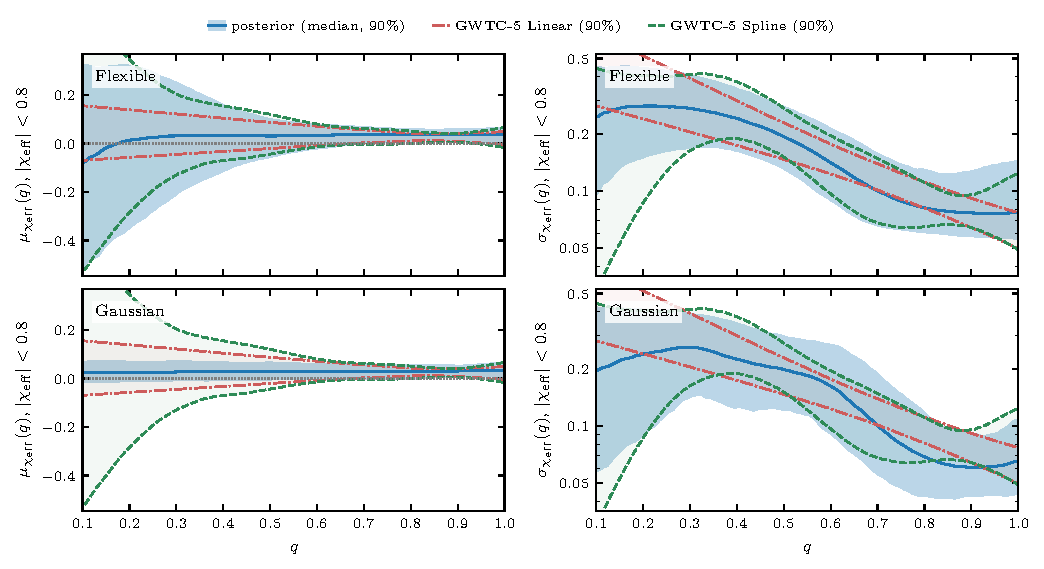
\includegraphics[width=\linewidth]{draft/plots/chi_eff_mean_sd_q_core_lvk.pdf}
    \caption{The mean (left) and width (right) of $\chieff$ as a function of mass ratio, as in Fig.~\ref{fig: width q}, with the GWTC-5 linear and spline $\chieff \mid q$ models.}
    \label{fig: mean width q}
\end{figure}

\begin{figure}
    \centering
    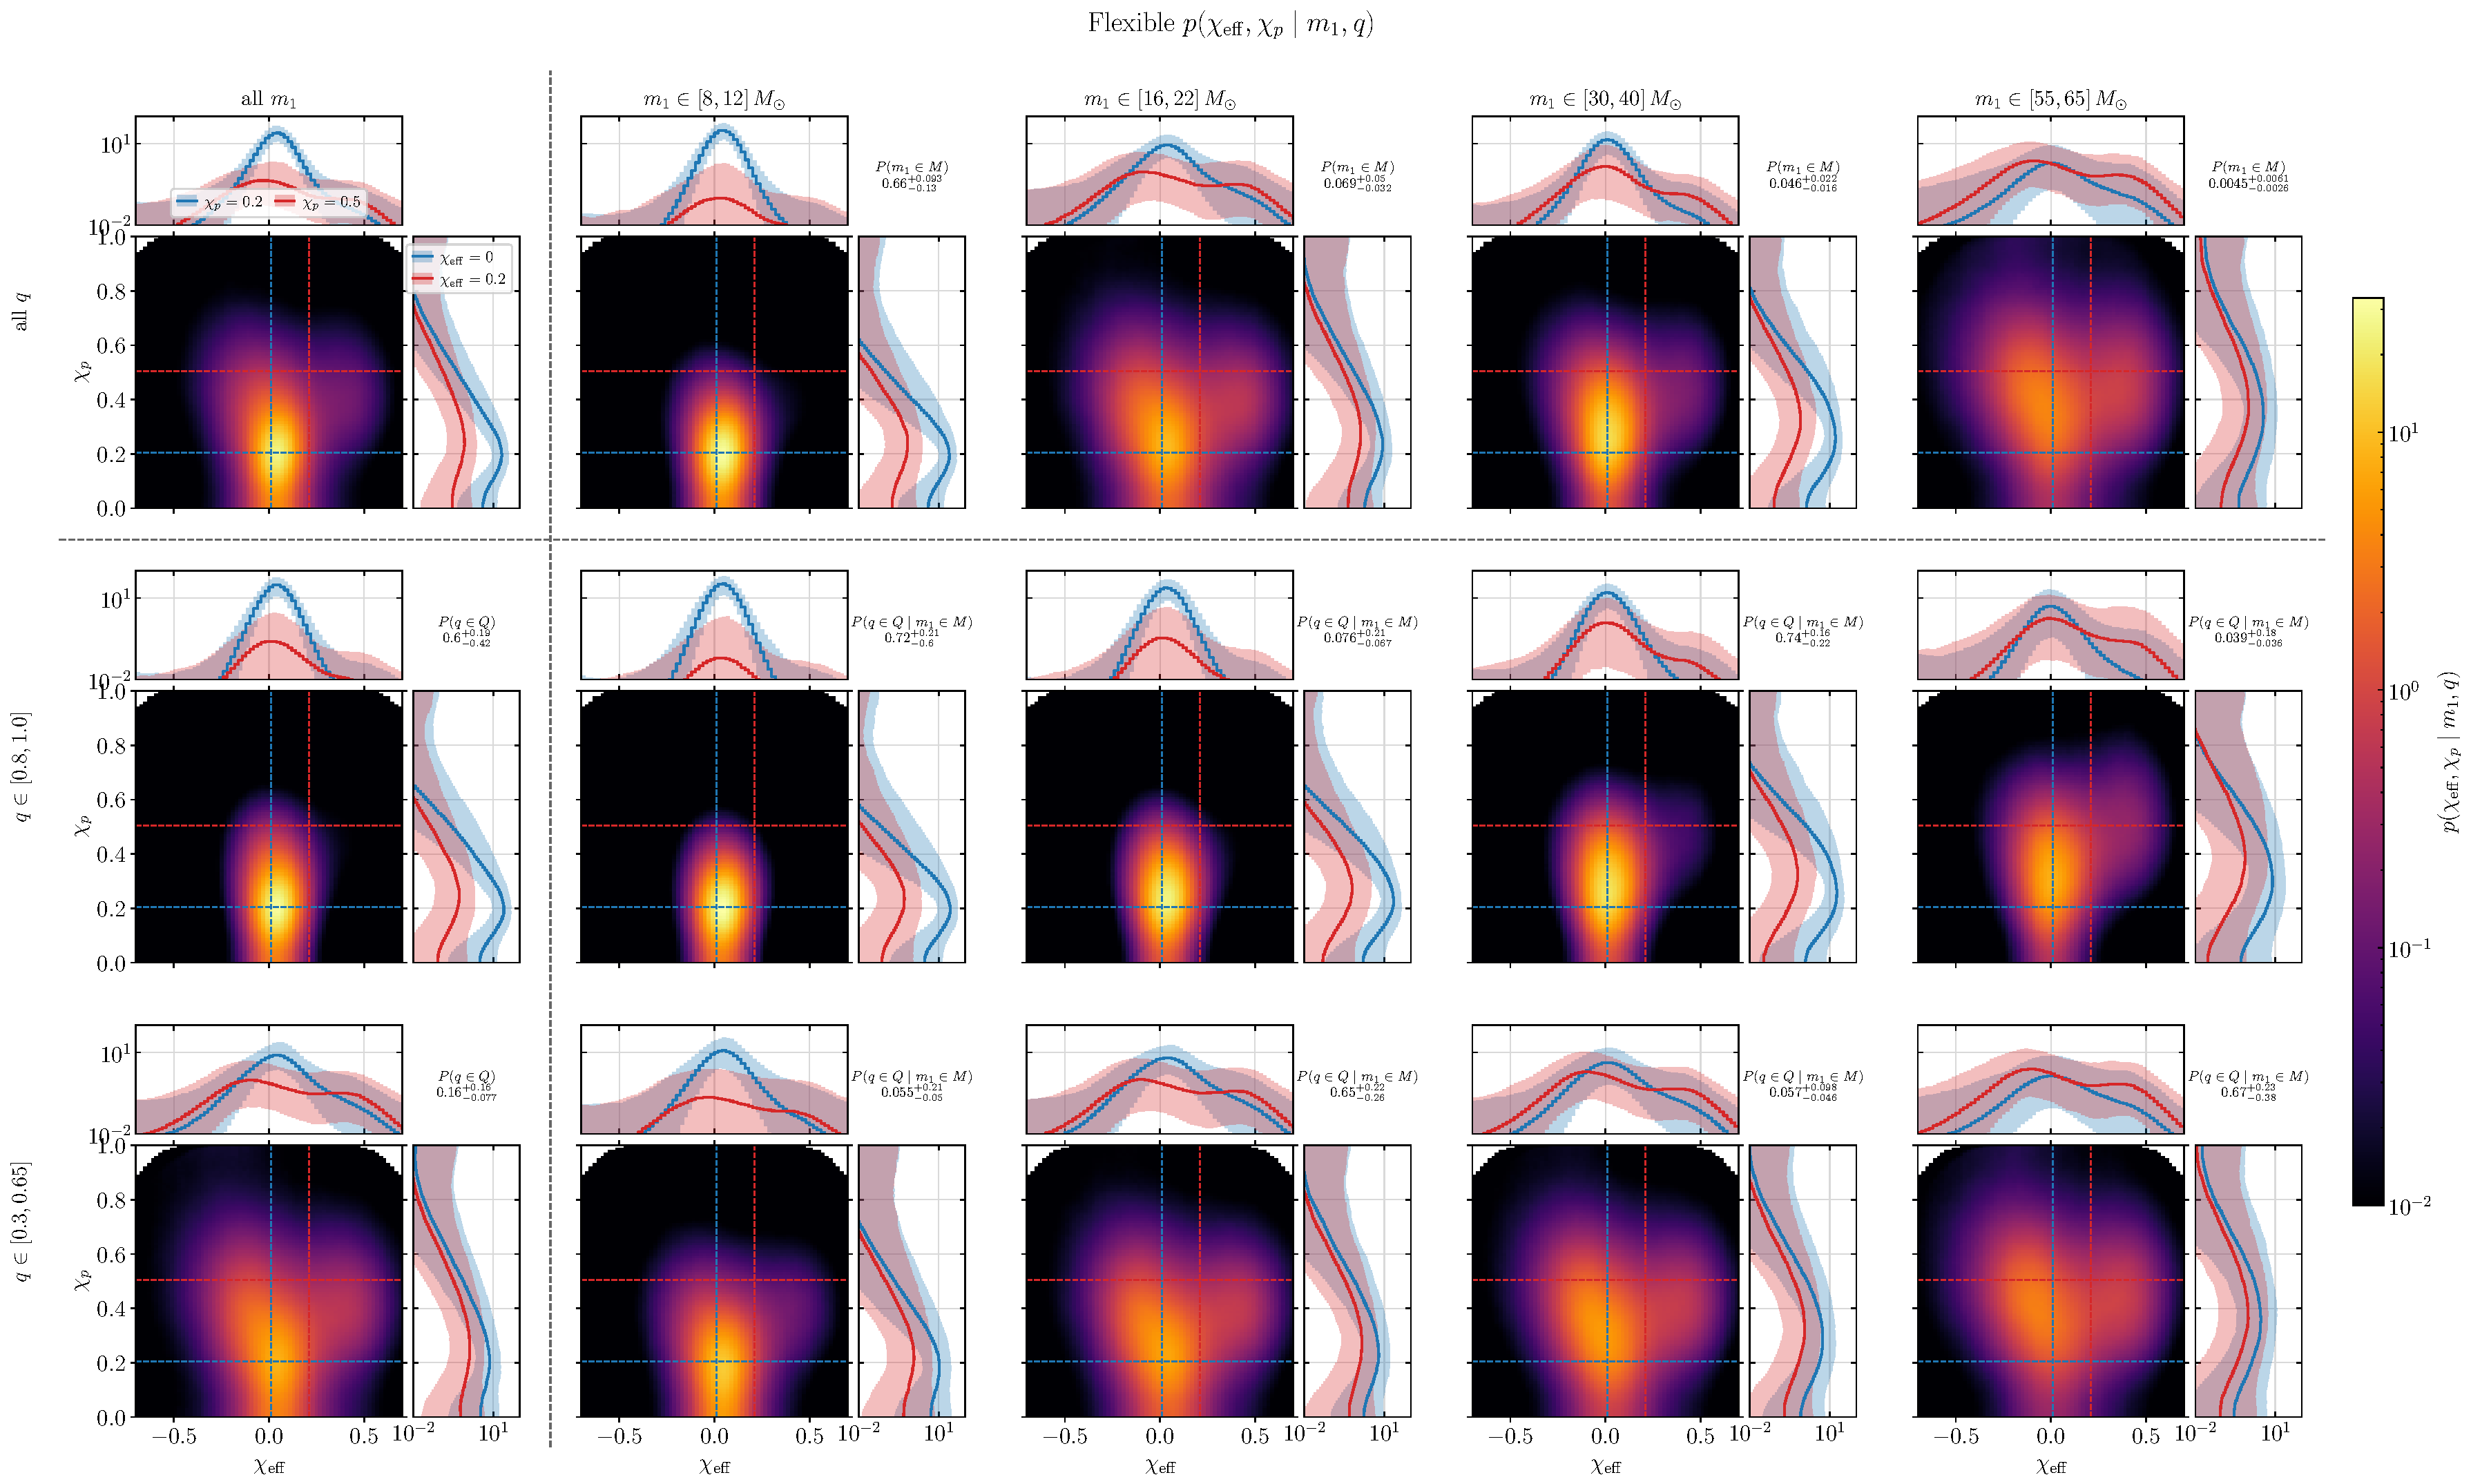
\includegraphics[width=\linewidth]{draft/plots/spin_regions_flexible.pdf}
    \caption{The joint spin distribution across the $(m_1, q)$ plane for the \flexiblespins model. \todo{caption}}
    \label{fig: regions flexible}
\end{figure}

\begin{figure}
    \centering
    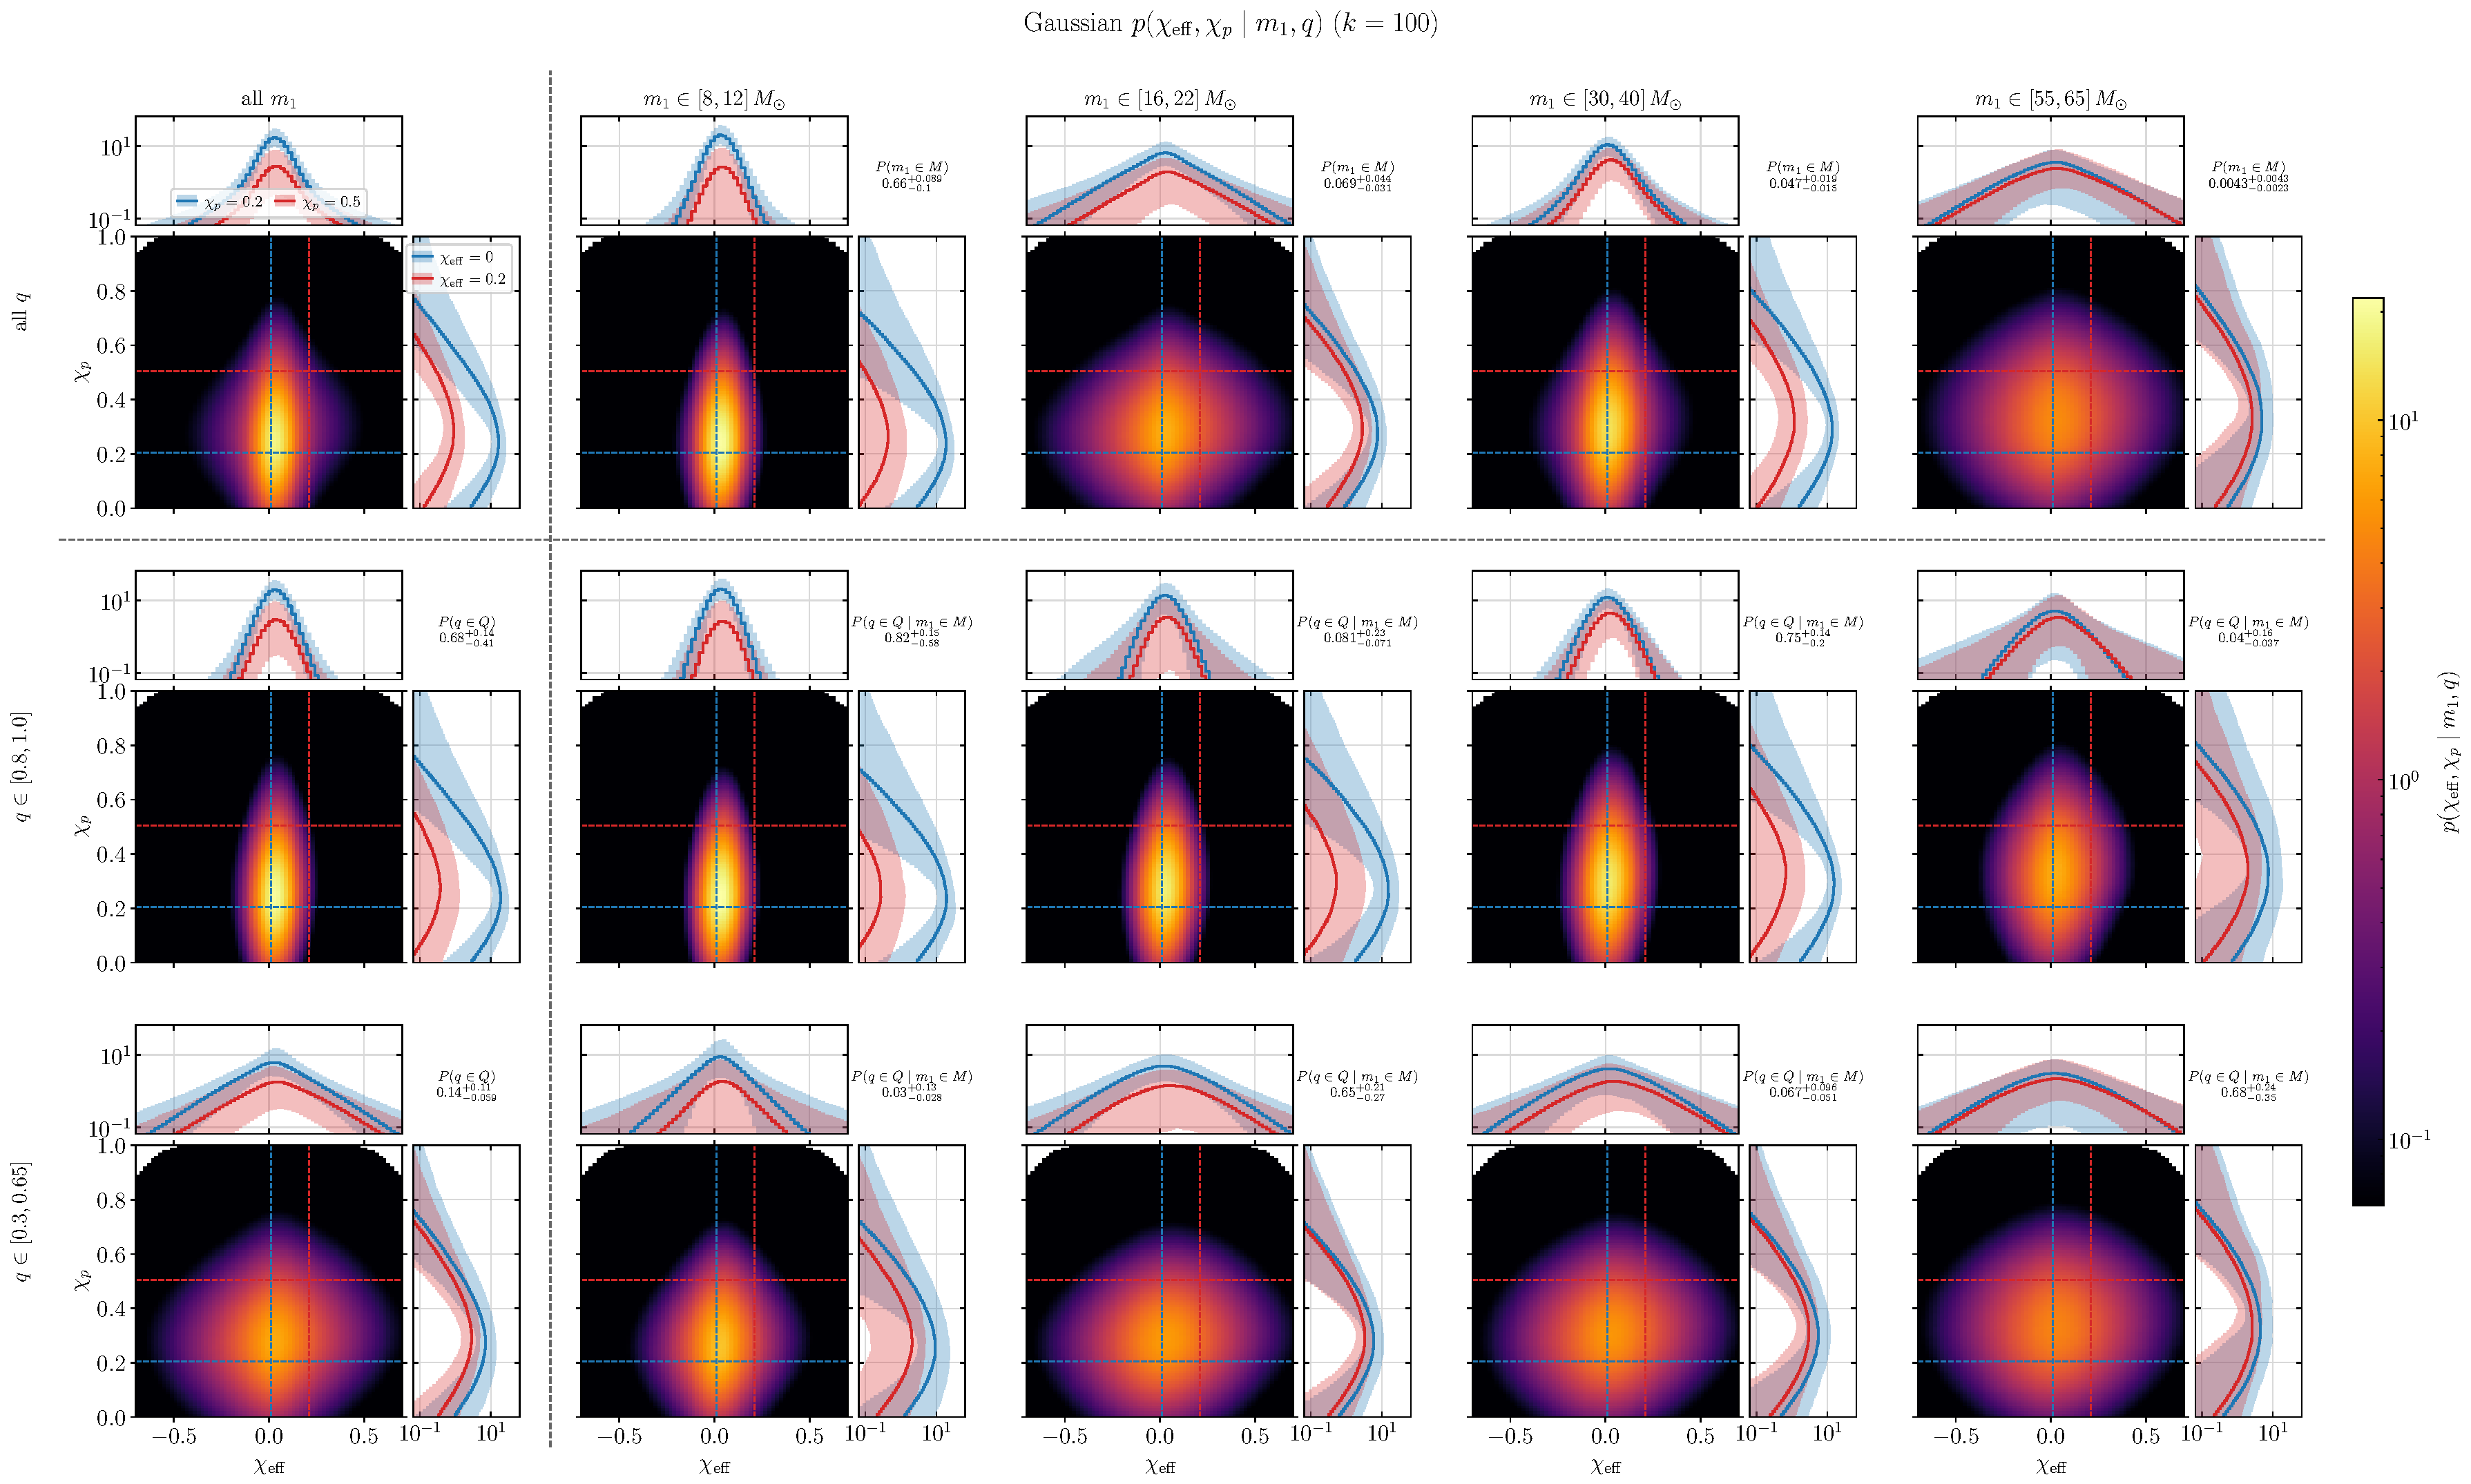
\includegraphics[width=\linewidth]{draft/plots/spin_regions_gaussian.pdf}
    \caption{As Fig.~\ref{fig: regions flexible}, for the \gaussianspins model.}
    \label{fig: regions gaussian}
\end{figure}

\end{document}
